\setchapterimage[8cm]{Paul Pastourmatzis Unsplash}
\setchapterpreamble[u]{\margintoc}
\chapter{概率论}
\labch{probability}

\section{集合理论}

概率论中的$\subset$可能表示包含关系,也可能表示真包含关系. 而$\subseteq$一定表示包含关系,$\subsetneq$一定表示真包含关系.

$\sigma$-代数又叫$\sigma$-域.

\begin{definition}[概率空间]
    设 $\Omega$ 为样本空间, $\mathscr{F}$ 为 $\Omega$ 的部分子集构成的 $\sigma$-代数. 如果存在定义在 $\mathscr{F}$ 上而取值于 $[0,1]$ 的函数 $P$ ,满足
    \begin{enumerate}[label=(\roman*)]
        \item 规范性: $P(\Omega)=1$;
        \item 可列可加性:对 $A_i \in \mathscr{F}, i=1,2, \cdots$ ,且 $A_i \cap A_j=\emptyset, i \neq j$ ,有
              $$
                  P\left(\bigcup_{i=1}^{\infty} A_i\right)=\sum_{i=1}^{\infty} P\left(A_i\right),
              $$
    \end{enumerate}
    则称 $\mathscr{F}$ 为事件域, $P$ 为概率, $P(A)$ 为事件 $A \in \mathscr{F}$ 的概率, 三元组 $(\Omega, \mathscr{F}, P)$ 为概率空间.
\end{definition}


\subsection{Dynkin 定理}

\begin{definition}[$\pi$-系统、$\sigma$-代数、$\lambda$-系统]
    设 $S$ 是一个非空集合, $\mathcal{P}(S):=\{A \subseteq S\}$ 是 $S$ 的幂集. 称集族 $\mathcal{A} \subseteq \mathcal{P}(S)$ 是一个 $S$ 上的
    \begin{enumerate}
        \item $\pi$-系统, 如果 $\mathcal{A}$ 对集合的有限交运算封闭, 即 $A, B \in \mathcal{A} \Longrightarrow A \cap B \in \mathcal{A}$.
        \item $\sigma$-代数, 如果
              \begin{enumerate}[label=(\roman*)]
                  \item $S \in \mathcal{A}$
                  \item $\mathcal{A}$ 对集合的补运算封闭,即 $A \in \mathcal{A} \Longrightarrow A^c \in \mathcal{A}$
                  \item $\mathcal{A}$ 对集合的可数交\sidenote{可以等价替换为可数并,因为$\sigma$-代数对补运算封闭}运算封闭,即对可数多个\sidenote[][*2]{这里的可数多个如果替换为有限个,那它就成了代数的定义. $\sigma$通常表示可数多个}集合 $A_1, A_2, \cdots \in \mathcal{A}$ ,我们有
                        $$
                            \bigcap_{i=1}^{\infty} A_i \in \mathcal{A} .
                        $$
              \end{enumerate}
        \item $\lambda$-系统, 如果\footnote{如果满足前两条,则称为$\lambda_0$类,我们有$\pi$类+$\lambda_0$类=代数,而条件三等价于单调类,于是$\pi$类+$\lambda_0$类+单调类=$\sigma$代数}
              \begin{enumerate}[label=(\roman*)]
                  \item \label{def:lambda_system_1}$S \in \mathcal{A}$\marginnote{$\lambda$-系统定义中的\ref{def:lambda_system_1},\ref{def:lambda_system_2}说明$\lambda$-系统对集合的补运算封闭}
                  \item \label{def:lambda_system_2}$A, B \in \mathcal{A}, A \subseteq B \Longrightarrow B \backslash A \in \mathcal{A}$
                  \item \sidenote{可以等价替换为:设$A_1\subseteq A_2\subseteq \cdots$是$\mathcal{A}$中的可数多项的升链,则$$\bigcup_{i=1}^{\infty} A_i \in \mathcal{A}$$}设 $A_1, A_2, \cdots \in \mathcal{A}$ 是可数多个互不相交的集合, 则有
                        $$
                            \bigsqcup_{i=1}^{\infty} A_i \in \mathcal{A}
                        $$
              \end{enumerate}
    \end{enumerate}
\end{definition}

\begin{theorem}[Dynkin $\pi$-$\lambda$ 定理]\label{thm:dynkin_pi_lambda_theorem}
    设$\mathcal{F}\subseteq \mathcal{P}(S)$是一个$\pi$-系统,则
    $$
        \sigma(\mathcal{F})=\lambda(\mathcal{F})
    $$
\end{theorem}

\begin{theorem}[单调类定理]\label{thm:monotone_class_theorem}
    设$\mathcal{F}\subseteq \mathcal{P}(S)$是一个代数,则
    $$
        \sigma(\mathcal{F})=M(\mathcal{F})
    $$
\end{theorem}

\begin{theorem}
    单调类定理\ref{thm:monotone_class_theorem} 与 Dynkin 定理\ref{thm:dynkin_pi_lambda_theorem} 是等价的.
\end{theorem}

接下来我们总结一下这些集合系统之间的关系:
\begin{itemize}
    \item 所有的 $\sigma$-代数 $\subseteq$ 所有的 $\lambda$-系统 $\subseteq$ 所有的单调类
    \item 所有的 $\sigma$-代数 $\subseteq$ 所有的代数 $\subseteq$ 所有的 $\pi$-系统
    \item $\sigma$-代数 $=$ 单调类 + 代数 $=$ $\lambda$-系统 + $\pi$-系统
\end{itemize}

\section{离散型与连续型随机变量}

\begin{definition}[离散型随机变量]
    如果随机变量$X$ 的取值为有限个或可数个,则称$X$为离散型随机变量.
\end{definition}

以下就$X$取可数个值的情况进行讨论. 有限值情况类似.

设$X$是离散型随机变量,取值为$x_1,x_2,\cdots,x_n,\cdots$,则$X$的分布列定义为
$$
    p_k=\mathbb{P}(X=x_k)
$$
设函数$f(x)$取值于$\{x_1,x_2,\cdots\}$,$f(x_k)=p_k$,则称$f(x)$为随机变量$X$的概率质量函数(PMF, Probability Mass Function).

当分布列 $\left\{p_k\right\}$ 的规律性不够明显时, 也常常用如下的方式表达概率分布,
\begin{tabular}{c|cccc}
    $X$       & $x_1$ & $x_2$ & $x_3$ & $\cdots$ \\
    \hline$P$ & $p_1$ & $p_2$ & $p_3$ & $\cdots$
\end{tabular}
分布列具有如下性质:
\begin{itemize}
    \item $p_k\ge 0$
    \item $\sum_{k=1}^{\infty} p_k=1$\sidenote{因为对于$k\ne j$,$\{X=x_j\}$发生,$\{X=x_k\}$就不能发生,所以$\{X=x_j\},j=1,2,\cdots$是互不相容事件. 利用
              \[
                  \Omega=\bigcup_{k=1}^{\infty} \{X=x_k\}
              \]
              和概率的可列可加性得到
              \[
                  1=\mathbb{P}(\Omega)=\sum_{k=1}^{\infty} \mathbb{P}(X=x_k)=\sum_{k=1}^{\infty} p_k
              \]
          }
\end{itemize}


\begin{definition}[连续型随机变量]
    设$X$是随机变量,如果存在非负函数$f(x)$使得对任何满足$-\infty\le a<b\le \infty$的$a,b$,有
    $$
        \mathbb{P}(a\le X\le b)=\int_a^b f(x) \, dx
    $$
    则称$X$为连续型随机变量. 称$f(x)$为$X$的概率密度函数.
\end{definition}

设$f(x)$是$X$的概率密度,则$f(x)$有如下的基本性质.
\begin{itemize}
    \item $\int_{-\infty}^{\infty} f(x) \, dx=1$
    \item 对任意$a\in\mathbb{R}$,有$\mathbb{P}(X=a)=0$,于是
          $$
              \mathbb{P}(a\le X\le b)=\mathbb{P}(a<X\le b)=\mathbb{P}(a\le X<b)=\mathbb{P}(a<X<b)
          $$
    \item 对数集$A\in\mathcal{R}$,有
          $$
              \mathbb{P}(X\in A)=\int_A f(x) \, dx
          $$
\end{itemize}

\section{独立性}

\begin{definition}[独立性]
    \begin{itemize}
        \item 两个事件$A,B$独立\footnote{若$A,B$独立,则$A^c,B$独立,$A,B^c$独立,$A^c,B^c$独立. 证明思路是将$A\cup B$看成全集再 Subtract.},当且仅当$\mathbb{P}(A\cap B)=\mathbb{P}(A)\mathbb{P}(B)$.\marginnote{事件$A,B$独立,当且仅当随机变量$\mathbb{1}_A,\mathbb{1}_B$独立}
        \item 两个随机变量$X,Y$独立\footnote{若$X,Y$独立,则$\sigma(X),\sigma(Y)$独立.},当且仅当对任意$C,D\in\mathcal{R}$,有$\mathbb{P}(X\in C, Y\in D)=\mathbb{P}(X\in C)\mathbb{P}(Y\in D)$.\sidenote{也就是说,事件$A=\{X\in C\}$与$B=\{Y\in D\}$独立}
        \item 两个$\sigma$-域$\mathcal{F},\mathcal{G}$独立,当且仅当对任意$A\in\mathcal{F}$,$B\in\mathcal{G}$,有$\mathbb{P}(A\cap B)=\mathbb{P}(A)\mathbb{P}(B)$.
    \end{itemize}
\end{definition}

\begin{kaobox}[frametitle="独立"与"两两独立"]
    对于事件$A_1,A_2,\cdots,A_n$,
    \begin{itemize}
        \item 独立\sidenote[][*-2]{即对于任意指标$I\subset \{1,2,\cdots,n\}$,有$\mathbb{P}\left(\bigcap_{i\in I}A_i\right)=\prod_{i\in I}\mathbb{P}(A_i)$}一定两两独立\sidenote{即$\mathbb{P}(A_i\cap A_j)=\mathbb{P}(A_i)\mathbb{P}(A_j)$对任意$i\ne j$成立}
        \item 两两独立不一定独立\sidenote[][*1]{反例考虑:设$X_1,X_2,X_3$是独立的随机变量,且$\mathbb{P}(X_i=0)=\mathbb{P}(X_i=1)=1/2$. 令$A_1=\{X_2=X_3\}$,$A_2=\{X_3=X_1\}$,$A_3=\{X_1=X_2\}$. 这些事件两两独立但不独立,因为$\mathbb{P}(A_1\cap A_2\cap A_3)=1/4\ne 1/8=\mathbb{P}(A_1)\mathbb{P}(A_2)\mathbb{P}(A_3)$}
    \end{itemize}
\end{kaobox}

\begin{definition}[集合类的独立]\label{def:集合类的独立}
    集合类$A_1,A_2,\cdots,A_n\in\mathcal{F}$被称为独立,如果对任意$A_i\in\mathcal{A}_i$和$I\subset \{1,2,\cdots,n\}$,有$\mathbb{P}(\bigcap_{i\in I}A_i)=\prod_{i\in I}\mathbb{P}(A_i)$.
\end{definition}

\begin{lemma}
    不失一般性,可以假设每个$\mathcal{A}_i$都包含全集$\Omega$. 那么定义\ref{def:集合类的独立}中等价于
    $$
        \mathbb{P}\left(\bigcap_{i\in I}A_i\right)=\prod_{i\in I}\mathbb{P}(A_i)\qquad \text{whenever } A_i\in\mathcal{A}_i\sidenote{因为对于$i\notin I$,可以令$A_i=\Omega$,这样就不用定义$I$了.}
    $$
\end{lemma}

\begin{theorem}\label{thm:independence_of_sigma_algebras}
    假设集合类$\mathcal{A}_1,\mathcal{A}_2,\cdots,\mathcal{A}_n$独立,且$\mathcal{A}_i$是$\pi$-系统,那么$\sigma(\mathcal{A}_1),\sigma(\mathcal{A}_2),\cdots,\sigma(\mathcal{A}_n)$也独立.
\end{theorem}

在数学中,想要证明某个性质对一个很大的集合成立,只需要证明这个性质对于集合的生成元成立即可. 如下的定理就利用了这个思想,目标是对于实数上的Borel代数成立,但是只需要对形如$\{(-\infty,a):a\in \mathbb{R}\}$的集合成立即可.\sidenote{甚至只需对$\{(-\infty,a):a\in \mathbb{Q}\}$证明成立即可. 因为一列可数个有理数可以逼近任意实数.}因为$\sigma(\{(-\infty,a):a\in \mathbb{R}\})=\mathcal{B}$.

\begin{theorem}
    为了证明$X_1,X_2,\cdots,X_n$独立,只需要证明:对于任意$x_1,x_2,\cdots,x_n\in (-\infty,\infty]$,有
    $$
        \mathbb{P}\left(\bigcap_{i=1}^n \{X_i\le x_i\}\right)=\prod_{i=1}^n \mathbb{P}(X_i\le x_i)
    $$
\end{theorem}

\begin{proof}
    令$\mathcal{A}_i$为形如$\{X_i\le x_i\}$的集合类,这显然是$\pi$-系统,由下面的练习\ref{ex:sigma_algebra_generated_by_inverse_image}可知,$\sigma(\mathcal{A}_i)=\sigma(X_i)$,所以根据定理\ref{thm:independence_of_sigma_algebras}就得到结果.
\end{proof}

\begin{exercise}\label{ex:sigma_algebra_generated_by_inverse_image}
    证明:若$\mathcal{A}$生成$\mathcal{S}$,那么$X^{-1}\coloneqq \{\{X\in A\}:A\in\mathcal{A}\}$生成$\sigma(X)=\{\{X\in B\}:B\in\mathcal{S}\}$.
\end{exercise}

\begin{proof}
    照章办事. 令$\mathcal{G}$是包含$X^{-1}(\mathcal{A})$的最小$\sigma$-代数. 因为$\sigma(X)$是包含$X^{-1}(\mathcal{A})$的$\sigma$-代数,所以$\sigma(X)\subseteq \mathcal{G}$. 职是之故,存在$\sigma$-域\sidenote{因为$\mathcal{G}$是$\sigma$-域.}$\mathcal{F}$满足$\mathcal{A}\subset \mathcal{F}\subset\mathcal{S}$,使得有$\mathcal{G}=\{\{X\in B\}:B\in\mathcal{S}\}$. 由于$\mathcal{S}$是由$\mathcal{A}$生成的,所以$\mathcal{F}=\mathcal{S}$.
\end{proof}

\begin{theorem}\label{thm:independence_of_sigma_algebras_2}
    令集合类\marginnote{这是二维的情况}$\mathcal{F}_{i,j},1\le i\le n,1\le j\le m(i)$独立,令$\mathcal{G}_i=\sigma(\cup_j\mathcal{F}_{i,j})$. 则$\mathcal{G}_1,\mathcal{G}_2,\cdots,\mathcal{G}_n$独立.
\end{theorem}

\begin{proof}
    令$\mathcal{A}_i$为具有形式$\cap_j A_{i,j}$的集合类(其中$A_{i,j}\in\mathcal{F}_{i,j}$),显然$\mathcal{A}_i$是$\pi$-系统,包含$\Omega$和$\cup_j\mathcal{F}_{i,j}$,所以根据定理\ref{thm:independence_of_sigma_algebras}就得到:$\sigma(\mathcal{A}_i)=\mathcal{G}_i$独立.
\end{proof}

\begin{theorem}\label{thm:independence_of_inverse_image}
    若$X_{i,j},1\le i\le n,1\le j\le m(i)$独立,$f_i:\mathbf{R}^{m(i)}\to \mathbf{R}$可测,那么$f_i(X_{i,1},X_{i,2},\cdots,X_{i,m(i)})$独立.
\end{theorem}

\begin{proof}
    令$\mathcal{F}_{i,j}=\sigma(X_{i,j})$,则$\mathcal{F}_{i,j}$独立,令$\mathcal{G}_i=\sigma(\cup_j\mathcal{F}_{i,j})$,则根据定理\ref{thm:independence_of_sigma_algebras_2},$\mathcal{G}_1,\mathcal{G}_2,\cdots,\mathcal{G}_n$独立,........未完待续\sidenote{没有搞懂这个证明.}
\end{proof}

定理\ref{thm:independence_of_inverse_image}的特殊情况是:若$X_1,X_2,\cdots,X_n$独立,则$X_1$与$X_2\cdots X_n$独立. 而且,$X_1+X_2+\cdots+X_n$与$X_1,X_2,\cdots ,X_n$独立.

\begin{exercise}
    若$(X_1,X_2,\cdots,X_n)$有概率密度$f(x_1,x_2,\cdots,x_n)$\sidenote{即对于任意$A\in\mathcal{R}^n$,有$$\mathbb{P}((X_1,X_2,\cdots,X_n)\in A)=\int_A f(x_1,x_2,\cdots,x_n) \, dx$$},且$f(x)$可以被写成$g(x_1)g(x_2)\cdots g(x_n)$,其中$g_m\ge 0$,则$X_1,X_2,\cdots,X_n$独立.\footnote{$g_m$并不必为概率密度函数.}
\end{exercise}

\begin{proposition}
    \begin{itemize}
        \item 设 $(\xi, \eta)$ 是离散型随机变量, 那么它们独立的充要条件是联合分布列等于两个边沿分布列的乘积.
        \item 设 $(\xi, \eta)$ 是连续型随机变量, 那么它们独立的充要条件是联合密度函数在其连续点上等于两个边沿密度函数的乘积.
    \end{itemize}
\end{proposition}

现在考虑下面的问题: 如果 $\xi, \eta$ 是随机变量, $f \in \mathscr{B}^2$. 问: 在求期望 $E[f(\xi, \eta)]$ 时, 能否先固定一个, 即先求 $E[f(x, \eta)]$, 得到 $x$ 的函数, 再将 $\xi$ 代入到这个函数中去, 得到一个随机变量,然后求这个随机变量的期望?\sidenote{回答一般是否定的. 例如,取 $f(x, y)=x y$ . 此时,对任意两个随机变量 $\xi, \eta$ ,上面公式成立意味着 $E[\xi \eta]=E[\xi] E[\eta]$ ,即 $\xi, \eta$ 不相关. 这显然一般是不对的. 比如, $\xi=\eta, \xi$ 是对称随机变量 $(\xi$ 与 $-\xi$ 同分布 $), E[\xi]=0$ (例如 $\xi \sim N(0,1))$. 则
$$
    \varphi(x):=E[x \eta]=0, \quad \forall x,
$$
于是
$$
    E[\varphi(\xi)]=0
$$
但显然
$$
    E[f(\xi, \eta)]=E\left[\xi^2\right] \neq 0
$$}

但是在独立的情形下, 这个结论是成立的. 我们有如下的定理:
\begin{theorem}\label{thm:independence_of_random_variables_and_expectation}
    设 $f: \mathbb{R}^2 \mapsto \mathbb{R}$ 为非负 Borel可测, $(\xi, \eta)$ 为二维随机变量. 令
    $$
        \varphi(x):=E[f(x, \eta)] .
    $$
    则 $\varphi: \mathbb{R} \mapsto \mathbb{R}$ 为非负 Borel可测,且 $\xi, \eta$ 为独立的充要条件对任意这样的 $f$,
    $$
        E[f(\xi, \eta)]=E[\varphi(\xi)] .
    $$
\end{theorem}
\begin{note}
    这个定理是条件期望的一个应用.
\end{note}
\begin{proof}
    先证$\varphi$的Borel可测性,由于非负可测函数可以由非负简单函数单调上升地逼近,所以由单调收敛定理,只需对$f$是非负简单函数证明. 而由期望的线性性,这又归结为对示性函数证明. 因此我们设
    \[f=1_A,\quad A\in\mathscr{B}^2\]
    令
    $$
        \mathscr{G}:=\left\{A \in \mathscr{B}^2: \varphi(x):=E\left[1_A(x, \eta)\right] \text { 为Borel可测 }\right\} .
    $$
    则易证 $\mathscr{G}$ 为 $\lambda$-类, 且包含了 $\pi$-类:
    $$
        \Pi:=\{(-\infty, a] \times(-\infty, b], a, b \in \mathbb{R}\} .
    $$
    因此由单调类定理有 $\mathscr{G}=\sigma(\Pi)=\mathscr{B}^2$.

    下面证第二个结论. 充分性显然,因为取
    $$
        f(x, y):=1_{(-\infty, a]}(x) \cdot 1_{(-\infty, b]}(y),
    $$
    则
    $$
        E[f(\xi, \eta)]=E[\varphi(\xi)]
    $$
    就变为
    $$
        P(\xi \leqslant a, \eta \leqslant b)=P(\xi \leqslant a) P(\eta \leqslant b) .
    $$
    往证必要性. 令
    $$
        \begin{gathered}
            \mathscr{G}:=\left\{A \in \mathscr{B}^2: \text { 定理对函数 } f:=1_A \text { 成立 }\right\} . \\
            \mathscr{C}:=\{(a, b] \times(c, d]: a<b, c<d\} .
        \end{gathered}
    $$
    则 $\mathscr{C}$ 为 $\pi$-类, 且 $\mathscr{B}^2=\sigma(\mathscr{C})$. 对 $A:=(a, b] \times(c, d] \in \mathscr{C}$, 令
    $$
        f:=1_A .
    $$
    则
    $$
        \varphi(x)=E\left[1_A(x, \eta)\right]=1_{(a, b]}(x) E\left[1_{(c, d]}(\eta)\right]=1_{(a, b]}(x) P(c<\eta \leqslant d) .
    $$
    所以
    $$
        E[\varphi(\xi)]=E\left[1_{(a, b]}(\xi)\right] P(c<\eta \leqslant d)=P(a<\xi \leqslant b) P(c<\eta \leqslant d) .
    $$
    而由独立性也有
    $$
        \begin{aligned}
            E[f(\xi, \eta)] & =E\left[1_{(a, b] \times(c, d]}(\xi, \eta)\right] \\
                            & =P(a<\xi \leqslant b, c<\eta \leqslant d)         \\
                            & =P(a<\xi \leqslant b) P(c<\eta \leqslant d) .
        \end{aligned}
    $$
    所以, $\mathscr{C} \subset \mathscr{G}$.

    往证 $\mathscr{G}$ 为 $\lambda$-类. 显然 $\mathbb{R}^2 \in \mathscr{G}$. 设 $A, B \in \mathscr{G}, A \subset B$. 对任意 $C \subset \mathscr{B}^2$, 令
    $$
        \varphi_C(x):=E\left[1_C(x, \eta)\right],
    $$
    则
    $$
        E\left[\varphi_B(\xi)\right]-E\left[\varphi_A(\xi)\right]=E\left[\varphi_{B \backslash A}(\xi)\right] .
    $$
    因此
    $$
        \begin{aligned}
            E\left[1_{B \backslash A}(\xi, \eta)\right] & =E\left[1_B(\xi, \eta)-1_A(\xi, \eta)\right]               \\
                                                        & =E\left[1_B(\xi, \eta)\right]-E\left[1_A(\xi, \eta)\right] \\
                                                        & =E\left[\varphi_B(\xi)\right]-E\left[\varphi_A(\xi)\right] \\
                                                        & =E\left[\varphi_{B \backslash A}(\xi)\right] .
        \end{aligned}
    $$
    所以 $B-A \in \mathscr{G}$. 再设 $A_n \in \mathscr{G}, A_n \uparrow A$. 则由单调收敛定理有
    $$
        \begin{aligned}
            E\left[1_A(\xi, \eta)\right] & =\lim _{n \rightarrow \infty} E\left[1_{A_n}(\xi, \eta)\right] \\
                                         & =\lim _{n \rightarrow \infty} E\left[\varphi_{A_n}(\xi)\right] \\
                                         & =E\left[\lim _{n \rightarrow \infty} \varphi_{A_n}(\xi)\right] \\
                                         & =E\left[\varphi_A(\xi)\right]
        \end{aligned}
    $$
    所以 $A \in \mathscr{G}$. 这样, 由 $\lambda-\pi$ 定理, $\mathscr{G}$ 为 $\sigma$-代数. 于是 $\mathscr{G}=\mathscr{B}^2$.

    现在, 若 $f$ 是简单函数:
    $$
        f:=\sum_{k=1}^n a_k 1_{A_k}, \quad a_k \in \mathbb{R}, A_k \in \mathscr{B}^2,
    $$
    则有
    $$
        \begin{aligned}
            E[f(\xi, \eta)] & =\sum_{k=1}^n a_k E\left[1_{A_k}(\xi, \eta)\right] \\
                            & =\sum_{k=1}^n a_k E\left[\varphi_{A_k}(\xi)\right] \\
                            & =E\left[\sum_{k=1}^n a_k \varphi_{A_k}(\xi)\right] \\
                            & =E[\varphi(\xi)]
        \end{aligned}
    $$
    最后, 设 $f \geqslant 0, f \in \mathscr{B}^2$. 于是, 存在简单函数 $f_n \uparrow f$. 以 $\varphi_n$ 表示 $f_n$ 对应的 $\varphi$, 则由单调收敛定理,有
    $$
        \begin{aligned}
            E[f(\xi, \eta)] & =\lim _{n \rightarrow \infty} E\left[f_n(\xi, \eta)\right] \\
                            & =\lim _{n \rightarrow \infty} E\left[\varphi_n(\xi)\right] \\
                            & =E[\varphi(\xi)]
        \end{aligned}
    $$
\end{proof}
在定理\ref{thm:independence_of_random_variables_and_expectation}中,用$f(x,y)\cdot \mathbb{1}_{f(x,y)\in A}$替换$f(x,y)$,则有
\begin{corollary}
    延续定理\ref{thm:independence_of_random_variables_and_expectation}中的符号,若 $\xi, \eta$ 独立,则
    \[
        \mathbb{P}(f(\xi,\eta)\in A)=\mathbb{E}[\varphi(\eta)]
    \]
    其中$\varphi(y)=\mathbb{P}(f(\xi,y)\in A)$
\end{corollary}

\section{不相关与独立}

对于随机变量$\xi,\eta$,若$\mathbb{E}[\xi\eta]=\mathbb{E}[\xi]\mathbb{E}[\eta]$,则称$\xi,\eta$不相关. 也就是说他们的协方差为0.

自然地,独立意味着不相关,但是不相关并不意味着独立. 因为不相关是个整体的概念\sidenote{求期望是整体概念},而独立是局部概念.

\begin{note}
    但在一个重要的特殊情形,不相关和独立是等价的. 这就是$(\xi,\eta)$服从二维正态分布的情形.
\end{note}

\begin{theorem}
    如果$(\xi,\eta)$服从二维正态分布,则$\xi,\eta$不相关当且仅当$\xi,\eta$独立.
\end{theorem}

\begin{theorem}
    设$\xi$和$\eta$均为只取两个不同值的随机变量,那么$\xi$与$\eta$独立的充要条件是它们不相关.
\end{theorem}

\begin{proof}
    只用证明不相关\sidenote{$E[\xi\eta]=E[\xi]E[\eta]$.}推出独立性,不妨设$\xi,\eta\in\{0,1\}$,直接解方程即可验证$P(\xi=i,\eta=j)=P(\xi=i)P(\eta=j),i,j\in\{0,1\}$.
    \[
        \begin{array}{c|c|c|c}
                & X=0                              & X=1 &     \\
            \hline
            Y=0 & \begin{array}{c} p_1 \end{array} & p_2 & a   \\
            \hline
            Y=1 & p_3                              & p_4 & 1-a \\
            \hline
                & b                                & 1-b &     \\
        \end{array}
    \]
    由不相关性,可以知道$E[XY]=E[X]E[Y]$,即$p_4=(1-a)(1-b)$. 显然可以求出$p_1,p_2,p_3$,从而验证独立性.
\end{proof}

\section{分布}

% \begin{definition}[分布函数、概率密度函数]\label{def:distribution_function_and_probability_density_function}

% \end{definition}
\subsection{特殊分布函数}

\begin{itemize}
    \item 均匀分布 $U(a,b)$: 分布函数与概率密度函数为
          $$f(x)=\begin{cases}
                  0,               & x<a       \\
                  \frac{x-a}{b-a}, & x\in[a,b] \\
                  1,               & x>b
              \end{cases} \qquad p(x)=\begin{cases}
                  \frac{1}{b-a}, & x\in[a,b] \\
                  0,             & \text{其他}
              \end{cases}$$
          特征函数为
          $$\varphi(t) = \frac{e^{itb} - e^{ita}}{it(b-a)}$$
    \item 指数分布 $Exp(\lambda)$: 分布函数与概率密度函数为
          $$f(x)=\begin{cases}
                  1-e^{-\lambda x}, & x\geq 0 \\
                  0,                & x<0
              \end{cases} \qquad p(x)=\begin{cases}
                  \lambda e^{-\lambda x}, & x\geq 0 \\
                  0,                      & x<0
              \end{cases}$$
          特征函数为
          $$\varphi(t) = \frac{\lambda}{\lambda - it}$$
    \item 正态分布 $N(\mu,\sigma^2)$: 分布函数与概率密度函数为
          \begin{gather*}
              f(x)=\frac{1}{\sqrt{2\pi}\sigma}\int_{-\infty}^x e^{-\frac{(t-\mu)^2}{2\sigma^2}}dt \\
              p(x)=\frac{1}{\sqrt{2\pi}\sigma}e^{-\frac{(x-\mu)^2}{2\sigma^2}}, \quad x\in\mathbb{R}
          \end{gather*}
          特征函数为
          $$\varphi(t) = e^{i\mu t - \frac{1}{2}\sigma^2 t^2}$$
    \item 二项分布 $B(n,p)$: 分布函数与概率质量函数为
          $$f(x)=\sum_{k\leq x}\binom{n}{k}p^k(1-p)^{n-k} \qquad P(X=k)=\binom{n}{k}p^k(1-p)^{n-k}, \quad k=0,1,\ldots,n$$
          特征函数为
          $$\varphi(t) = \left(q + pe^{it}\right)^n, \quad q = 1-p$$
    \item 泊松分布 $P(\lambda)$: 分布函数与概率质量函数为
          $$f(x)=\sum_{k\leq x}\frac{\lambda^k}{k!}e^{-\lambda} \qquad P(X=k)=\frac{\lambda^k}{k!}e^{-\lambda}, \quad k=0,1,2,\ldots$$
          特征函数为
          $$\varphi(t) = e^{\lambda(e^{it} - 1)}$$
    \item 几何分布 $G(p)$: 分布函数与概率质量函数为
          $$f(x)=1-(1-p)^{\lfloor x \rfloor} \qquad P(X=k)=p(1-p)^{k-1}, \quad k=1,2,\ldots$$
          特征函数为
          $$\varphi(t) = \frac{pe^{it}}{1 - (1-p)e^{it}}$$
    \item 超几何分布 $H(N,M,n)$: 分布函数与概率质量函数为
          $$f(x)=\sum_{k\leq x}\frac{\binom{M}{k}\binom{N-M}{n-k}}{\binom{N}{n}} \qquad P(X=k)=\frac{\binom{M}{k}\binom{N-M}{n-k}}{\binom{N}{n}}, \quad k=\max(0,n-N+M),\ldots,\min(n,M)$$
          特征函数较复杂,通常不以简单形式表示。
    \item 负二项分布 $NB(r,p)$: 分布函数与概率质量函数为
          $$f(x)=\sum_{k\leq x}\binom{k+r-1}{k}p^r(1-p)^k \qquad P(X=k)=\binom{k+r-1}{k}p^r(1-p)^k, \quad k=0,1,2,\ldots$$
          特征函数为
          $$\varphi(t) = \left(\frac{p}{1 - (1-p)e^{it}}\right)^r$$
\end{itemize}

\begin{theorem}[gamma 分布的性质]
    若$X\sim gamma(\alpha,\lambda),Y=gamma(\beta,\lambda)$,且$X,Y$独立,则$X+Y\sim gamma(\alpha+\beta,\lambda)$.\footnote{证明只需照章办事,}
\end{theorem}

\begin{theorem}[正态分布的性质]
    若$X\sim normal(\mu ,a ),Y\sim normal(\nu,b)$,且$X,Y$独立,则$X+Y\sim normal(\mu+\nu,a+b)$.\footnote{证明只需照章办事.}
\end{theorem}

目前我们接触到的分布的关系为
\begin{itemize}
    \item $n$ 个独立同分布 $B(1, p)$ 的 0-1 分布随机变量之和服从二项分布 $B(n, p)$
    \item 若 $X_1\sim B(n_1,p),X_2\sim B(n_2,p)$ 且独立,则 $X_1+X_2\sim B(n_1+n_2,p)$
    \item 若 $X_1\sim P(\lambda_1),X_2\sim P(\lambda_2)$ 且独立,则 $X_1+X_2\sim P(\lambda_1+\lambda_2)$
    \item $r$ 个独立同分布几何分布 $G(p)$ 的随机变量之和服从参数为 $r$ 和 $p$ 的 Pascal 分布
    \item 若 $X_i\sim N(\mu_i,\sigma_i^2),i=1,\cdots,n$ 且独立,则对任意实数 $a_1,\cdots,a_n$,有
          $$\sum_{i=1}^n a_iX_i\sim N\left(\sum_{i=1}^n a_i\mu_i,\sum_{i=1}^n a_i^2\sigma_i^2\right)$$
\end{itemize}

\subsection{联合分布与边缘分布}
对于随机向量 $(X, Y)$, 我们称
$$
    F(x, y)=P(X \leq x, Y \leq y)
$$
为 $(X, Y)$ 的联合概率分布函数, 简称为联合分布 (joint distribution).
$$
    \begin{gathered}
        F_X(x)=P(X \leq x, Y \leq \infty)=F(x, \infty) \\
        F_Y(y)=P(X \leq \infty, Y \leq y)=F(\infty, y)
    \end{gathered}
$$
我们称 $X$ 的分布函数 $F_X(x)$, $Y$ 的分布函数 $F_Y(x)$ 为 $(X, Y)$ 的边缘分布函数 (marginal distribution function).

\begin{theorem}
    设 $X, Y$ 分别有概率密度 $f_X(x), f_Y(y)$. 则 $X, Y$ 独立的充分必要条件是随机向量 $(X, Y)$ 有联合密度
    $$
        f(x, y)=f_X(x) f_Y(y) .
    $$
\end{theorem}

\subsection{二维正态分布}
特别地,设 $(\xi, \eta)$ 服从二维正态分布 $N(\mu, \Sigma)$ ,其中 $\mu=\left(\mu_1, \mu_2\right)$ ,
$$
    \Sigma=\left(\begin{array}{cc}
            \sigma_1^2             & \rho \sigma_1 \sigma_2 \\
            \rho \sigma_1 \sigma_2 & \sigma_2^2
        \end{array}\right)
$$
其中 $\sigma_1, \sigma_2>0, \rho \in(-1,1)$ .则 $(\xi, \eta)$ 的密度函数写成分量形式为
$$
    \begin{aligned}
        p(x, y)= & \frac{1}{2 \pi \sigma_1 \sigma_2 \sqrt{1-\rho^2}} \exp \left\{-\frac{1}{2\left(1-\rho^2\right)}\right.                                                                                       \\
                 & \left.\cdot\left[\frac{\left(x-\mu_1\right)^2}{\sigma_1^2}-\frac{2 \rho\left(x-\mu_1\right)\left(y-\mu_2\right)}{\sigma_1 \sigma_2}+\frac{\left(y-\mu_2\right)^2}{\sigma_2^2}\right]\right\}
    \end{aligned}
$$
此时,也记为 $(\xi, \eta) \sim N\left(\mu_1, \mu_2, \sigma_1^2, \sigma_2^2, \rho\right)$ .图\ref{fig:二维正态分布}是 $N(5,5,1,1,0.5)$ 的密度函数图像.
\begin{marginfigure}
    \centering
    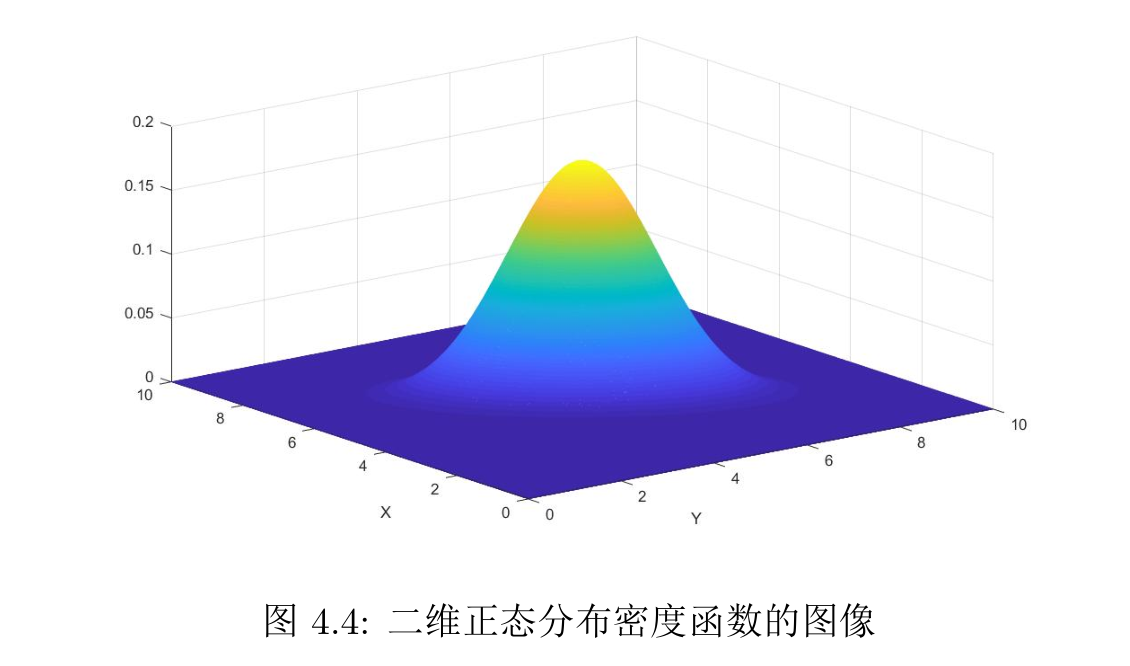
\includegraphics[width=\textwidth]{二维正态分布.png}
    \caption{二维正态分布的密度函数图像}
    \label{fig:二维正态分布}
\end{marginfigure}
现在求其边沿分布.为此将 $p(x, y)$ 改写为
$$
    \begin{aligned}
        p(x, y)= & \frac{1}{\sqrt{2 \pi} \sigma_1} \exp \left\{-\frac{\left(x-\mu_1\right)^2}{2 \sigma_1^2}\right\}                                                                                                                     \\
                 & \cdot \frac{1}{\sqrt{2 \pi\left(1-\rho^2\right)} \sigma_2} \exp \left\{-\frac{\left[y-\left(\mu_2+\rho \frac{\sigma_2}{\sigma_1}\left(x-\mu_1\right)\right]^2\right.}{2 \sigma_2^2\left(1-\rho^2\right)}\right\}     \\
        =        & \frac{1}{\sqrt{2 \pi} \sigma_2} \exp \left\{-\frac{\left(y-\mu_2\right)^2}{2 \sigma_2^2}\right\}                                                                                                                     \\
                 & \cdot \frac{1}{\sqrt{2 \pi\left(1-\rho^2\right)} \sigma_1} \exp \left\{-\frac{\left[x-\left(\mu_1+\rho_{\frac{\sigma_1}{\sigma_2}}\left(y-\mu_2\right)\right)\right]^2}{2 \sigma_1^2\left(1-\rho^2\right)}\right\} .
    \end{aligned}
$$
由此易得
$$
    \begin{aligned}
         & p_{\xi}(x)=\int_{\mathbb{R}} p(x, y) d y=\frac{1}{\sqrt{2 \pi} \sigma_1} e^{-\frac{\left(x-\mu_1\right)^2}{2 \sigma_1^2}}, \\
         & p_\eta(y)=\int_{\mathbb{R}} p(x, y) d x=\frac{1}{\sqrt{2 \pi} \sigma_2} e^{-\frac{\left(y-\mu_2\right)^2}{2 \sigma_2^2}} .
    \end{aligned}
$$
这就是说,正态分布的边沿分布仍为正态分布,$\xi \sim N\left(\mu_1, \sigma_1^2\right)$ 和 $\eta \sim N\left(\mu_2, \sigma_2^2\right)$ .注意这两个边沿分布都与 $\rho$ 无关,这就顺带举出了一个不同的联合分布有相同的边沿分布的例子.
\begin{example}
    如果$(\alpha,\beta)\sim N(0,0,1,1,0.5)$,$(\xi,\eta)\sim (0,0,1,1,-0.5)$那么 $(\alpha,\beta)$ 和 $(\xi,\eta)$ 的边沿分布相同,但联合分布不同.
\end{example}

同时,由于两个边缘分布$N(\mu_1,\sigma_1^2)$和$N(\mu_2,\sigma_2^2)$的协方差$\operatorname{Cov}(\xi,\eta)=\rho\sigma_1\sigma_2$,所以当相关系数$\rho=0$的时候,即不相关,$\xi$和$\eta$独立. 

\section{随机变量的函数的分布}

最简单的情形,是由一维随机变量 $X$ 的概率分布去求其一给函数 $Y=g(X)$ 的分布. 较常见的,是由 $\left(X_1, X_2, \cdots, X_n\right)$ 的分布求 $Y=g\left(X_1, X_2, \cdots, X_n\right)$ 的分布. 更一般地,由 $\left(X_1, X_2, \cdots, X_n\right)$的分布去求 $\left(Y_1, Y_2, \cdots, Y_m\right)$ 的分布,其中 $Y_i=g_i\left(X_1, X_2, \cdots, X_n\right)$ $i=1,2, \cdots, m$ .

这一部分内容,与数理统计中求统计量的分布有密切的联系.

\subsection{离散型随机变量的情形}

设$X$的分布律为
\[
    P(X=x_i)=p_i, \quad i=1,2,\cdots
\]
令$g:\mathbb{R}\to\mathbb{R}$,则$Y=g(X)$的分布律为
\[
    P(Y=y_j)=P(g(X)=y_j)=\sum_{x_i;g(x_i)=y_j}p_i=\sum_{i:g(x_i)=y_j}p_i
\]
上述结论可以推广到多维随机变量的情况.

设随机向量$X$的分布律为$P(X=x)$,则$X$的函数$Y=g(X)$的分布律为
\[
    P(Y=y)=P(g(X)=y)=\sum_{x:g(x)=y}p(X=x)
\]
\begin{example}
    设 $X \sim B(n, p), Y \sim B(m, p)$ 且 $X$ 和 $Y$ 相互独立,则 $X+Y \sim$ $B(n+m, p)$.
\end{example}
这种性质叫做\textbf{再生性}. 可推广至多维.\sidenote{再生性的证明可以考虑使用特征函数,会更加简单.}
\begin{example}
    设 $X \sim P(\lambda), Y \sim P(\mu)$ , 且 $X$ 和 $Y$ 独立,则有 $X+Y \sim$ $P(\lambda+\mu)$ . 即 Poisson 分布亦具有再生性.
\end{example}

\subsection{连续型随机变量的情形}

\begin{theorem}[密度变换公式]
    设随机变量$X$有概率密度函数$f(x),x\in(a,b)(a,b$可以为$\infty)$, 而$y=g(x)$在$x\in(a,b)$上是严格单调的连续函数,存在唯一的反函数$x=h(y),y\in(\alpha,\beta)$并且$h^{\prime}(y)$存在且连续, 那么$Y=g(X)$也是连续型随机变量且有概率密度函数
    $$
        p(y)=f(h(y))\left|h^{\prime}(y)\right|, \quad y\in(\alpha,\beta).
    $$
\end{theorem}

\begin{remark}
    当 $g$ 不是在全区间上单调而是逐段单调时, 密度变换公式变为逐段的:
    $$
        p(y)=\sum_{i=1}^n f(h_i(y))\left|h_i^{\prime}(y)\right|, \quad y\in(\alpha,\beta).
    $$
    其中$h_i(y)$是$g(x)=y$在$x\in(a_i,b_i)$上的唯一解,$a_i,b_i$是$g(x)$的单调区间.
\end{remark}
接下来是多维随机变量的情况.
\begin{theorem}[二维密度变换公式]\label{eq:two-dimensional_density_transform}
    设 $\left(\xi_1, \xi_2\right)$ 是 2 维连续型随机向量,具有联合密度函数 $p\left(x_1, x_2\right)$ ,设 $\zeta_j=f_j\left(\xi_1, \xi_2\right), j=1,2$ . 若 $\left(\xi_1, \xi_2\right)$ 与 $\left(\zeta_1, \zeta_2\right)$ 一一对应,逆映射 $\xi_j=h_j\left(\zeta_1, \zeta_2\right), j=1,2$ . 假定每个 $h_j\left(y_1, y_2\right)$ 都有一阶连续偏导数. 则 $\left(\zeta_1, \zeta_2\right)$ 亦为连续型随机向量,且其联合概率密度为
    $$
        q\left(y_1, y_2\right)=\left\{\begin{array}{cl}
            p\left(h_1\left(y_1, y_2\right), h_2\left(y_1, y_2\right)\right)|J|, & \left(y_1, y_2\right) \in \mathbb{D}    \\
            0,                                                                   & \left(y_1, y_2\right) \notin \mathbb{D}
        \end{array}\right.
    $$
    其中 $\mathbb{D}$ 是随机向量 $\left(\zeta_1, \zeta_2\right)$ 的所有可能值的集合, $J$ 是变换的 Jaccobi行列式,即
    $$
        J=\left|\begin{array}{ll}
            \frac{\partial h_1}{\partial y_1} & \frac{\partial h_1}{\partial y_2} \\
            \frac{\partial h_2}{\partial y_1} & \frac{\partial h_2}{\partial y_2}
        \end{array}\right|
    $$
\end{theorem}

\begin{theorem}[n维密度变换公式]\label{eq:n-dimensional_density_transform}
    设 $\left(\xi_1, \cdots, \xi_n\right)$ 是 $n$ 维连续型随机向量, 具有联合密度函数 $p\left(x_1, \cdots, x_n\right)$ . 假设存在 $n$ 个 $n$ 元函数
    $$
        y_j=f_j\left(x_1, \cdots, x_n\right), \quad j=1, \cdots, n
    $$
    使得
    $$
        \zeta_j=f_j\left(\xi_1, \cdots, \xi_n\right), \quad j=1, \cdots, n
    $$
    若 $\left(\xi_1, \cdots, \xi_n\right)$ 与 $\left(\zeta_1, \cdots, \zeta_n\right)$ 之间一一对应,逆映射为 $\xi_j=h_j\left(\zeta_1, \cdots, \zeta_n\right)$ , $j=1, \cdots, n$ . 其中每个 $h_j\left(y_1, \cdots, y_n\right)$ 都有一阶连续偏导数,那么随机向量 $\left(\zeta_1, \cdots, \zeta_n\right)$ 是连续型的,且具有联合密度函数
    $$
        q\left(y_1, \cdots, y_n\right)=\left\{\begin{array}{cl}
            p\left(h_1\left(y_1, \cdots, y_n\right), \cdots, h_n\left(y_1, \cdots, y_n\right)\right)|J|, & \left(y_1, \cdots, y_n\right) \in \mathbb{D}    \\
            0,                                                                                           & \left(y_1, \cdots, y_n\right) \notin \mathbb{D}
        \end{array}\right.
    $$
    其中 $\mathbb{D}$ 是随机向量 $\left(\zeta_1, \cdots, \zeta_n\right)$ 的所有可能值的集合, $J$ 是变换的 Jaccobi行列式,即
    $$
        J=\left|\begin{array}{ccc}
            \frac{\partial h_1}{\partial y_1} & \cdots & \frac{\partial h_1}{\partial y_n} \\
            \vdots                            & \ddots & \vdots                            \\
            \frac{\partial h_n}{\partial y_1} & \cdots & \frac{\partial h_n}{\partial y_n}
        \end{array}\right|
    $$
    其中 $\mathbb{D}$ 是随机向量 $\left(\zeta_1, \cdots, \zeta_n\right)$ 的所有可能值的集合, $J$ 是变换的 Jaccobi 行列式, 即
    $$
        J=\left|\begin{array}{ccc}
            \frac{\partial h_1}{\partial y_1} & \cdots & \frac{\partial h_1}{\partial y_n} \\
            \vdots                            & \vdots & \vdots                            \\
            \frac{\partial h_n}{\partial y_1} & \cdots & \frac{\partial h_n}{\partial y_n}
        \end{array}\right|
    $$
\end{theorem}
一些连续型随机变量,也具有再生性.
\begin{example}
    设 $X \sim N\left(\mu_1, \sigma_1^2\right), Y \sim N\left(\mu_2, \sigma_2^2\right)$ 且 $X$ 与 $Y$ 相互独立, 则:
    $$
        X+Y \sim N\left(\mu_1+\mu_2, \sigma_1^2+\sigma_2^2\right) .
    $$
    更一般地, 设 $X_i \sim N\left(\mu_i, \sigma_i^2\right), i=1, \cdots, n, X_1, \cdots, X_n$ 相互独立. $a_1, \cdots, a_n, b$ 为任意 $n+1$ 个实数,其中 $a_1, \cdots, a_n$ 不全为零. 令 $X=\sum_{i=1}^n a_i X_i+b$, 则有: $X \sim N\left(\mu, \sigma^2\right)$, 其中 $\mu=\sum_{i=1}^n a_i \mu_i+b$, $\sigma^2=\sum_{i=1}^n a_i^2 \sigma_i^2$.
\end{example}
\begin{example}
    设 $X_1 \sim \chi_n^2, X_2 \sim \chi_m^2$, 且 $X_1$ 和 $X_2$ 相互独立, 则 $X_1+X_2 \sim$ $\chi_{n+m}^2$.
\end{example}
有时我们还会碰到计算随机变量之商的概率密度. 我们有
\begin{theorem}
    如果 $(\xi, \eta)$ 是二维连续型随机向量,它们的联合密度为 $f(x, y)$ ,则它们的商 $\xi / \eta$ 是连续型随机变量,具有密度函数
    $$
        \begin{aligned}
            p_{\frac{\xi}{\eta}}(x)             & =\int_{-\infty}^{\infty}|t| f(x t, t) d t, \quad \forall x \in \mathbb{R} . \\
            \text { 而 } p_{\frac{\eta}{\xi}}(x) & =\int_{-\infty}^{\infty}|u| f(u, x u) d u, \quad \forall x \in \mathbb{R} .
        \end{aligned}
    $$
\end{theorem}



\section{卷积}

分布函数$F_1$和$F_2$的卷积定义为
$$
    F(x)=\int_{-\infty}^{\infty} F_1(x-y)F_2(y) \, dy,\quad x\in\mathbb{R}
$$
写作
$$
    F=F_1*F_2
$$
简单验证可以知道$F$也是分布函数.
\begin{theorem}
    若$X_1,X_2$独立,则$X_1+X_2$的分布函数为$F_{X_1+X_2}=F_{X_1}*F_{X_2}$.
\end{theorem}
\begin{proof}
    我们希望证明
    \[\forall x\in\mathbb{R}, \quad \mathbb{P}(X_1+X_2\le x)=\mathbb{P}(X_1\le x-X_2)=F_{X_1}(x-X_2)\]
    为此我们定义函数
    \[f(x_1,x_2)=\begin{cases}
            1, & x_1+x_2\le x \\
            0, & \text{其他}
        \end{cases}\]
    则$f$是$\mathbb{R}^2$上的Borel可测函数,且
    \begin{align*}
        \int_\Omega f(X_1,X_2) \, d\mathbb{P} & =\iint_{\mathbb{R}^2} f(x_1,x_2) \, \mu^2(dx_1,dx_2)                    \\
                                              & =\int_{\mathbb{R}}\mu_2(dx_2)\int_{\mathbb{R}}f(x_1,x_2) \, \mu_1(dx_1) \\
                                              & =\int_{\mathbb{R}}\mu_2(dx_2)\int_{(-\infty,x-x_2)}1 \, \mu_1(dx_1)     \\
                                              & =\int_{-\infty}^{\infty}F_2(x-x_2) \, dF_1(x_2)                         \\
                                              & =F_1*F_2(x)
    \end{align*}
    这就是$\mathbb{P}(X_1+X_2\le x)=(F_1*F_2)(x)$.
\end{proof}
\begin{corollary}
    双算子$*$满足交换律和结合律.
\end{corollary}
概率密度函数$p_1$和$p_2$的卷积定义为
$$
    p(x)=\int_{-\infty}^{\infty} p_1(x-y)p_2(y) \, dy,\quad x\in\mathbb{R}
$$
写作
$$
    p=p_1*p_2
$$
简单验证可以知道$p$也是概率密度函数.
\begin{theorem}
    两个绝对连续的分布函数(概率密度分别为$p_1$和$p_2$)的卷积也是绝对连续的分布函数(概率密度为$p_1*p_2$).
\end{theorem}
\begin{proof}
    由Fubini定理,我们有
    \begin{align*}
        \int_{-\infty}^x p(u)du & =\int_{-\infty}^x du \int_{-\infty}^{\infty} p_1(u-y)p_2(y) \, dy                   \\
                                & = \int_{-\infty}^{\infty}\left[\int_{-\infty}^{x} p_1(u-y) \, du\right]p_2(y) \, dy \\
                                & = \int_{-\infty}^{\infty} F_1(x-y)p_2(y) \, dy                                      \\
                                & = \int_{-\infty}^{\infty} F_1(x-y) \, dF_2(y)                                       \\
                                & = (F_1*F_2)(x)
    \end{align*}
    也就是说,$p$是$F_1*F_2$的分布函数.
\end{proof}

两个概率测度$\mu_1$和$\mu_2$的卷积定义为
$$
    \mu(A)=\int_{\mathbb{R}^2} \mu_1(A-y) \, d\mu_2(y),\quad A\in\mathcal{B}(\mathbb{R}^2)
$$
写作
$$
    \mu=\mu_1*\mu_2
$$
简单验证可以知道$\mu$也是概率测度.

对于关于$\mu_1*\mu_2$可积的Borel函数$g$,我们有
\[
    \int_{\mathbb{R}} g(u)(\mu_1*\mu_2)(du)=\iint_{\mathbb{R}^2} g(x+y) \, \mu_1(dx)\mu_2(dy)
\]



\section{期望与方差}

\subsection{期望}

\begin{definition}[期望]
    设 $X$ 是有概率密度 $f(x)$ 的随机变量, 如果下式成立,
    $$
        \int_{-\infty}^{\infty}|x| f(x) d x<\infty
    $$
    就称
    $$
        \int_{-\infty}^{\infty} x f(x) d x
    $$
    为 $X$ 或 $f(x)$ 的数学期望或均值.
\end{definition}

期望具有如下性质:

设$\mathbb{E}|X_j|<\infty(1\leq j\leq n)$,$c_0,c_1,\cdots,c_n$是常数,则有以下结果:
\begin{enumerate}
    \item 线性组合$Y=c_0+c_1X_1+c_2X_2+\cdots+c_nX_n$的数学期望存在,且
          $$\mathbb{E}(Y)=c_0+c_1\mathbb{E}(X_1)+c_2\mathbb{E}(X_2)+\cdots+c_n\mathbb{E}(X_n)$$
    \item 若$X_1,X_2,\cdots,X_n$相互独立,则$Z=X_1X_2\cdots X_n$的数学期望存在,且
          $$\mathbb{E}(X_1X_2\cdots X_n)=\mathbb{E}(X_1)\mathbb{E}(X_2)\cdots\mathbb{E}(X_n)$$
    \item 若$X_1\leq X_2$,则$\mathbb{E}(X_1)\leq\mathbb{E}(X_2)$
\end{enumerate}

\begin{lemma}
    若$\mathbb{E}|X|=0$,则$P(X=0)=1$.
\end{lemma}

\begin{proof}
    \begin{align*}
        P(|X|>1/n) & =P(n|X|>1) \mathbb{E}(\mathbb{1}_{n|X|>1})           \\
                   & \le  E(n|X|\mathbb{1}_{n|X|>1}) \le n\mathbb{E}|X|=0
    \end{align*}
    由概率的连续性得到
    \[
        P(|X|>0)=P(\bigcap_{n=1}^{\infty} \{|X|>1/n\})=0
    \]
    所以$P(X=0)=1-P(|X|>0)=1$.
\end{proof}
以概率$1$发生又称为几乎必然(almost surely)发生,用a.s.表示.

\begin{definition}[中心矩和原点矩]
    设 $X$ 是随机变量, $m$ 是正整数. 如果 $\mathbb{E}|X|^m<\infty$, 就称
    \[
        \mathbb{E}X^m
    \]
    为 $X$ 的 $m$ 阶原点矩, 称
    \[
        \mathbb{E}(X-\mathbb{E}X)^m
    \]
    为 $X$ 的 $m$ 阶中心矩. 当 $m>2$ 时, 我们将原点矩和中心矩统称为高阶矩.
\end{definition}

\subsection{方差}

\begin{definition}[方差]
    设随机变量$X$的数学期望$\mu=\mathbb{E}X$有限,则称$\mathbb{E}(X-\mu)^2$为$X$的方差(variance),记作$\operatorname{Var}(X)$或$\sigma_{XX}$。当$\operatorname{Var}(X)<\infty$时,称$X$的方差有限。称$\sigma_X=\sqrt{\operatorname{Var}(X)}$为$X$的标准差(standard deviation)。
\end{definition}
当 $X$ 有概率密度 $f(x)$ 时, 利用公式 (2.1) 得到
$$
    \operatorname{Var}(X)=\int_{-\infty}^{\infty}(x-\mu)^2 f(x) d x .
$$
方差具有如下性质:

设$a,b,c$是常数,$\mathbb{E}(X)=\mu, \operatorname{Var}(X)<\infty,\mu_j=\mathbb{E}X_j,\operatorname{Var}(X_j)<\infty(1\le j\le n)$,则
\begin{enumerate}
    \item $\operatorname{Var}(a+bX)=b^2\operatorname{Var}(X)$
    \item $\operatorname{Var}(X)=\operatorname{E}(X-\mu)^2<\mathbb{E}(X-c)^2$,只要$c\ne \mu$\sidenote{
              \begin{align*}
                  \mathbb{E}(X-c)^2 & =\mathbb{E}(X-\mu+c-\mu)^2                                         \\
                                    & =\mathbb{E}(X-\mu)^2+2(c-\mu)\mathbb{E}(X-\mu)+\mathbb{E}(c-\mu)^2 \\
                                    & =\operatorname{Var}(X)+2(c-\mu)^2
              \end{align*}
          }
    \item $\operatorname{Var}(X)=0$的充分必要条件是$P(X=\mu)=1$
    \item $\operatorname{Var}(\sum_{j=1}^n X_j)=\sum_{i=1}^n \sum_{j=1}^n \operatorname{Cov}(X_i,X_j)=\sum_{i=1}^n \sum_{j=1}^n [\mathbb{E}(X_iX_j)-\mathbb{E}(X_i)\mathbb{E}(X_j)]$
    \item 当$X_1,\cdots,X_n$独立时,$\operatorname{Var}(\sum_{j=1}^n X_j)=\sum_{j=1}^n \operatorname{Var}(X_j)$
\end{enumerate}

\section{协方差}

设 $\sigma_X=\sqrt{\sigma_{X X}}, \sigma_Y=\sqrt{\sigma_{Y Y}}$ 分别是 $X, Y$ 的标准差.

\begin{definition}[协方差]
    设$\mu_X=\mathbb{E}X,\mu_Y=\mathbb{E}Y$存在,当$\mathbb{E}|(X-\mu_X)(Y-\mu_Y)|<\infty$时,称
    \[
        \mathbb{E}[(X-\mu_X)(Y-\mu_Y)]
    \]
    为随机变量$X,Y$的协方差(covariance)\footnote{$\operatorname{Cov}(X,Y)=\mathbb{E}(XY)-\mathbb{E}X\mathbb{E}Y$},记作$\operatorname{Cov}(X,Y)$或$\sigma_{XY}$。当$\operatorname{Cov}(X,Y)=0$时,称$X,Y$不相关。
\end{definition}

\begin{definition}[相关系数]
    当$0<\sigma_X\sigma_Y<\infty$时,称
    \[
        \rho_{XY}=\frac{\sigma_{XY}}{\sigma_X\sigma_Y}
    \]
    为$X,Y$的相关系数(correlation coefficient)。有时也用$\rho(X,Y)$表示相关系数$\rho_{XY}$。
\end{definition}
\begin{itemize}
    \item $|\rho_{XY}|\le 1$
    \item $|\rho_{XY}|=1$当且仅当存在$a,b\in\mathbb{R}$,使得$P(Y=aX+b)=1$
    \item 若$X,Y$独立,则$X,Y$不相关,即$\rho_{XY}=0$.
\end{itemize}
\begin{example}
    设$(X,Y)$在单位圆$D=\{(x,y)\mid x^2+y^2\le 1\}$内均匀分布,则$X,Y$不相关,也不独立。
\end{example}
\begin{proof}
    由例2.4知道$\mathbb{E}(X)=\mathbb{E}(Y)=0$,于是
    \[
        \operatorname{Cov}(X,Y)=\iint_{\mathbb{R}^2} xy f(x,y)\,dx\,dy=\frac{1}{\pi}\int_{-1}^1 y\,dy\int_{-\sqrt{1-y^2}}^{\sqrt{1-y^2}} x\,dx=0
    \]
    所以$X,Y$不相关。

    又由$\S 3.3$的例3.1知道联合密度不能写成两个边缘密度的乘积,所以$X,Y$不独立。
\end{proof}
\begin{remark}
    相关系数$\rho_{XY}$只表示了$X,Y$间的线性关系。当$\rho_{XY}=0$时,尽管称$X,Y$不相关,它们之间还可以有很强的非线性关系。

    例如当$Y=X^2,X\sim N(0,\sigma^2)$时,$(X,Y)$总在抛物线$y=x^2$上,但是$X,Y$不相关,因为
    \[
        \operatorname{Cov}(X,Y)=\mathbb{E}[X(Y-\sigma^2)]=\mathbb{E}X^3-\sigma^2\mathbb{E}X=0
    \]
\end{remark}

\subsection{随机向量与随机矩阵的期望}

\begin{itemize}
    \item 设 $\boldsymbol{X}=\left(X_1, X_2, \ldots, X_n\right)$ 是随机向量, 若 $\mathrm{E} X_i=\mu_i$, 则记
          $$
              \boldsymbol{\mu}=\left(\mu_1, \mu_2, \ldots, \mu_n\right)
          $$
          称
          $$
              \mathrm{E} \boldsymbol{X}=\boldsymbol{\mu}
          $$
    \item 若 $Y_{i j}(i=1, \ldots, m, j=1, \ldots, n)$ 是随机变量, $\mathrm{E} Y_{i j}$ 存在, 记
          $$
              \boldsymbol{Y}=\left(\begin{array}{cccc}
                      Y_{11}  & Y_{12}  & \cdots & Y_{1 n} \\
                      Y_{21}  & Y_{22}  & \cdots & Y_{2 n} \\
                      \vdots  & \vdots  &        & \vdots  \\
                      Y_{m 1} & Y_{m 2} & \cdots & Y_{m n}
                  \end{array}\right)
          $$
          则称
          $$
              \mathrm{E} \boldsymbol{Y}=\left(\begin{array}{cccc}
                      \mathrm{E} Y_{11}  & \mathrm{E} Y_{12}  & \cdots & \mathrm{E} Y_{1 n} \\
                      \mathrm{E} Y_{21}  & \mathrm{E} Y_{22}  & \cdots & \mathrm{E} Y_{2 n} \\
                      \vdots             & \vdots             &        & \vdots             \\
                      \mathrm{E} Y_{m 1} & \mathrm{E} Y_{m 2} & \cdots & \mathrm{E} Y_{m n}
                  \end{array}\right)
          $$
\end{itemize}
设 $\boldsymbol{X}$ 和 $\boldsymbol{Y}$ 如上定义, $\mathrm{E} \boldsymbol{X}$ 和 $\mathrm{E} \boldsymbol{Y}$ 存在。
对任意常数向量 $\boldsymbol{a}=\left(a_1, \ldots, a_n\right), k \times m$ 常数矩阵 $A$ 和 $n \times l$ 常数矩阵 $B$, 有
$$
    \begin{aligned}
        \mathrm{E}\left(a \boldsymbol{X}^T\right) & =a \mathrm{E} \boldsymbol{X}^T,           \\
        (\mathrm{E} \boldsymbol{Y})^T             & =\mathrm{E}\left(\boldsymbol{Y}^T\right), \\
        \mathrm{E}(A \boldsymbol{Y})              & =A \mathrm{E}(\boldsymbol{Y}),            \\
        \mathrm{E}(\boldsymbol{Y} B)              & =\mathrm{E}(\boldsymbol{Y}) B,            \\
        \mathrm{E}(A \boldsymbol{Y} B)            & =A \mathrm{E}(\boldsymbol{Y}) B .
    \end{aligned}
$$

\subsection{协方差阵}
\begin{definition}[协方差矩阵]
    如果随机向量 $\boldsymbol{X}=\left(X_1, X_2, \cdots, X_n\right)$ 的数学期望 $\boldsymbol{\mu}=\mathrm{E} \boldsymbol{X}$存在,每个 $X_i$ 的方差 $\operatorname{Var}\left(X_i\right)<\infty$ ,就称
    $$
        \Sigma=\mathrm{E}\left[(\boldsymbol{X}-\boldsymbol{\mu})^{\mathrm{T}}(\boldsymbol{X}-\boldsymbol{\mu})\right]=\left(\sigma_{i j}\right)_{n \times n}
    $$
    为 $\boldsymbol{X}$ 的协方差矩阵. 其中
    $$
        \sigma_{i j}=\operatorname{Cov}\left(X_i, X_j\right)
    $$
    是 $X_i, X_j$ 的协方差.
    协方差矩阵 $\Sigma$ 是对称矩阵.
    如果矩阵 $A$ 的行列式 $\operatorname{det}(A)=0$, 就称 $A$ 是退化的.
\end{definition}
\begin{theorem}
    设 $\Sigma$ 是 $\boldsymbol{X}=\left(X_1, X_2, \cdots, X_n\right)$ 的协方差矩阵, 则
    \begin{enumerate}
        \item $\Sigma$ 是非负定矩阵,
        \item $\Sigma$ 退化的充分必要条件是有不全为零的常数 $a_1, a_2, \cdots, a_n$ 使得
              $$
                  P\left(\sum_{i=1}^n a_i\left(X_i-\mu_i\right)=0\right)=1
              $$
              其中 $\mu_i=\mathrm{E} X_i$.
    \end{enumerate}
\end{theorem}

\begin{proof}
    任取一个 $n$ 维实向量 $\boldsymbol{a}=\left(a_1, a_2, \cdots, a_n\right)$, 有
    $$
        \begin{aligned}
            \boldsymbol{a} \Sigma \boldsymbol{a}^{\mathrm{T}} & =\sum_{i=1}^n \sum_{j=1}^n a_i a_j \sigma_{i j}                                                        \\
                                                              & =\sum_{i=1}^n \sum_{j=1}^n a_i a_j \mathrm{E}\left[\left(X_i-\mu_i\right)\left(X_j-\mu_j\right)\right] \\
                                                              & =\mathrm{E}\left[\sum_{i=1}^n \sum_{j=1}^n a_i a_j\left(X_i-\mu_i\right)\left(X_j-\mu_j\right)\right]  \\
                                                              & =\mathrm{E}\left[\sum_{i=1}^n a_i\left(X_i-\mu_i\right)\right]^2                                       \\
                                                              & =\operatorname{Var}\left[\sum_{i=1}^n a_i\left(X_i-\mu_i\right)\right]                                 \\
                                                              & \geq 0 .
        \end{aligned}
    $$
    所以 $\Sigma$ 非负定.

    从上式看出, $\Sigma$ 退化的充分必要条件是有非零向量 $\boldsymbol{a}$ 使得
    $$
        \operatorname{Var}\left[\sum_{i=1}^n a_i\left(X_i-\mu_i\right)\right]=0
    $$
    再用定理 3.1 的(3)得到本定理的(2)。
\end{proof}

\section{条件期望与条件方差}

\begin{definition}[条件期望]
    $X:\Omega\to \mathbb{R}$是$(\Omega,\mathcal{F}_0,\mathbb{P})$上的随机变量,$X$可积\sidenote{即$\mathbb{E}|X|<\infty$.} $\mathcal{F}\subseteq \mathcal{F}_0$是$\sigma$-子域. 则称随机变量$Y:\Omega\to \mathbb{R}$为$X$在$\mathcal{F}$上的条件期望,满足:
    \begin{enumerate}
        \item $Y$是$\mathcal{F}$-可测
        \item 对于任意$A\in\mathcal{F}$,有$\mathbb{E}(X\mathbb{1}_A)=\mathbb{E}(Y\mathbb{1}_A)$
    \end{enumerate}
    我们将$Y$记为$\mathbb{E}(X|\mathcal{F})$.\footnote{$Y$存在唯一.}
\end{definition}

\begin{property}
    令$(\Omega,\mathcal{F},\mathbb{P})$是一个概率空间,$\mathcal{F}\subseteq \mathcal{F}_0$是一个$\sigma$-子域. 令$X,Y$是$\mathcal{F}$上的可积随机变量. 则
    \begin{enumerate}
        \item 对于任意$a,b\in\mathbb{R}$,有$\mathbb{E}(aX+bY|\mathcal{F})=a\mathbb{E}(X|\mathcal{F})+b\mathbb{E}(Y|\mathcal{F})$.
        \item 若$X\le Y$,则$\mathbb{E}(X|\mathcal{F})\le \mathbb{E}(Y|\mathcal{F})\, a.s.$
        \item 若$X_n\ge 0$且$X_n\uparrow X$,则$\mathbb{E}(X_n|\mathcal{F})\uparrow \mathbb{E}(X|\mathcal{F})$.
        \item 若$\sigma(X)$和$\mathcal{F}$独立,则$\mathbb{E}(X|\mathcal{F})=\mathbb{E}(X)$.
        \item 若$X\in\mathbb{F}$,则$\mathbb{E}(X|\mathcal{F})=X$.
    \end{enumerate}
\end{property}

\section{估计与放缩}

\begin{lemma}
    若$\displaystyle Y\geq0$,$\displaystyle p>0$,那么
    $$
        \mathbb{E}(Y^{p})=\int_{0}^{\infty} py^{p-1}\mathbb{P}(Y>y) \, dy\marginnote{经常用到的是:对于非负随机变量 $\displaystyle X$,有
            $$E[X]=\int_{0}^{\infty} \mathbb{P}(X>x) \, dx$$
        }
    $$
\end{lemma}

分布积分即可得到
\[
    \mathbb{E}(Y^{p})=\int_{0}^{\infty} x^{p} \, dF(x)=\int_{0}^{\infty} x^{p} f(x) \, dx
\]
其中$F(x)$是$Y$的分布函数,$f(x)$是$Y$的概率密度函数.

\begin{proposition}[Jensen 不等式]\label{prop:jensen_inequality}
    令$\varphi(x)$是$\mathbb{R}$上的凸函数\footnote{即对任意$x,y\in\mathbb{R}$,有$\varphi(\lambda x+(1-\lambda)y)\le \lambda \varphi(x)+(1-\lambda)\varphi(y)$},$X$是$\Omega$上的可积随机变量,且$\varphi(X)$也可积,则
    $$
        \varphi(\mathbb{E}X)\le \mathbb{E}(\varphi(X))
    $$
\end{proposition}

\begin{theorem}[Chebyshev 不等式]
    令$\varphi:\mathbf{R}\to\mathbf{R}$满足$\varphi\ge 0$,令$A\in\mathcal{R}$,$i_A\coloneqq \inf\{\varphi(y):y\in A\}$,则
    $$
        i_A \mathbb{P}(X\in A)\le \mathbb{E}(\varphi(X);X\in A)\le \mathbb{E}(\varphi(X))\marginnote{
            经常用到的版本是
            $$
                a^2\mathbb{P}(|X|\ge a)\le \mathbb{E}(X^2)
            $$
            只需令$A=\{x:|x|\ge a\}$,$\varphi(x)=x^2$即可.
        }
    $$
\end{theorem}

\begin{proof}
    考虑对应的随机变量版本:由$i_A$的定义和$\varphi\ge 0$可知
    $$
        i_A \mathbb{1}_{(X\in A)}\le \varphi(X)\mathbb{1}_{(X\in A)}\le \varphi(X)
    $$
    取期望即得结果.
\end{proof}

\begin{theorem}[Ottaviani 不等式]
    设有正常数$a,b$,使得对于任意$1\le k\le n$,有
    \[
        P(|S_n-S_k|\le b)\ge a
    \]
    则对任意$c>0$,
    \[
        P(\max_{1\le k\le n}|S_k-S_k|> b+c)\le \frac{1}{a}P(|S_n-S_k|>c)
    \]
\end{theorem}

\begin{proof}
    令\marginnote{$\tau$也就是$|S_k|$第一次超过$b+c$的时刻}
    \begin{gather}
        \tau\coloneqq \inf\{k:|S_k-S_k|>b+c\} \\
        A_k\coloneqq \{|S_k-S_k|\le b\}
    \end{gather}
    则$\{\tau =k\},k=1,2,\cdots,n$两两无交,且
    \begin{gather}
        \sum_{k=1}^n \{\tau =k\}=\left\{\max_{1\le k\le n}|S_k|>b+c\right\}\\
        \sum_{k=1}^n \{\tau =k\}A_k\subset \{|S_n|>c\}
    \end{gather}
    由于$\{\tau=k\}\in\sigma(\xi_1,\cdots,\xi_k),A_k\in\sigma(\xi_{k+1},\cdots,\xi_n)$,所以$\{\tau=k\}$与$A_k$独立,于是
    \begin{align*}
        P(|S_n|>c) & \ge P(\sum_{k=1}^n \{\tau =k\}A_k)  \\
                   & = \sum_{k=1}^n P(\{\tau =k\})P(A_k) \\
                   & \ge a\sum_{k=1}^n P(\{\tau =k\})    \\
                   & =aP(\max_{1\le k\le n}|S_k|>b+c)
    \end{align*}
\end{proof}

\begin{theorem}[Kolmogorov 不等式]\label{thm:kolmogorov_inequality}
    设 $\xi_1, \xi_2, \cdots, \xi_n$ 是相互独立随机变量, $E\left[\xi_i\right]=0, \forall i$. 记 $S_k:=\xi_1+\cdots+\xi_k$. 证明Kolmogorov不等式
    $$
        P\left(\max _{1 \leqslant k \leqslant n}\left|S_k\right| \geqslant C\right) \leqslant \frac{E\left[S_n^2\right]}{C^2} .
    $$
\end{theorem}

\begin{theorem}[广义 Kolmogorov 不等式]\label{thm:generalized_kolmogorov_inequality}
    条件和符号与定理\ref{thm:kolmogorov_inequality}相同. 证明: 若 $\varphi$ 还是非负偶函数, 且在正半轴上是递增的, 则
    $$
        P\left(\max _{1 \leqslant k \leqslant n} \varphi\left(S_k\right) \geqslant \varepsilon\right) \leqslant \frac{1}{\varphi(\varepsilon)} E\left[\varphi\left(S_n\right)\right], \quad \forall \varepsilon>0 .
    $$
    这就是广义Kolmogorov不等式.\footnote{取 $\varphi(x):=x^2$ 则得到本来的Kolmogorov不等式}
\end{theorem}
\begin{theorem}[Doob不等式]
    对 $p>1$ 有
    $$
        E\left[\left(\max _{1 \leqslant k \leqslant n}\left|S_k\right|\right)^p\right] \leqslant q^p E\left[\left|S_n\right|^p\right],
    $$
    其中 $1 / p+1 / q=1$. 此不等式称为Doob不等式.
\end{theorem}
\begin{exercise}\label{ex:1}
    设$X,Y$为随机变量,$EX=EY=0,DX=DY=1$,证明:$\forall \varepsilon>0$,有
    \[
        E(\max(X^2,Y^2))\le 1+\sqrt{1-\rho^2}
    \]
\end{exercise}
\begin{proof}
    \begin{align*}
            & E(\max(X^2,Y^2))                                                 \\
        =   & E\left(\frac{1}{2}(|X^2|+|Y^2|)+\frac{1}{2}|X^2-Y^2|\right)      \\
        =   & \frac{1}{2}E(|X^2|)+\frac{1}{2}E(|Y^2|)+\frac{1}{2}E(|X^2-Y^2|)  \\
        =   & \frac{1}{2}D(X)+\frac{1}{2}D(Y)+\frac{1}{2}E(|X-Y|)E(|X+Y|)      \\
        \le & 1+\frac{1}{2}\sqrt{E(|X-Y|^2)E(|X+Y|^2)}                         \\
        =   & 1+\frac{1}{2}\sqrt{(E(X^2)+E(Y^2)-2E(XY))(E(X^2)+E(Y^2)+2E(XY))} \\
        =   & 1+\frac{1}{2}\sqrt{4(1-\rho^2)}=1+\sqrt{1-\rho^2}
    \end{align*}
\end{proof}
\begin{corollary}
    对于任意给定的$\varepsilon>0$,有\footnote{其中$\sigma_X=\sqrt{DX},\sigma_Y=\sqrt{DY}$,$\rho$是$X,Y$的相关系数}
    \[
        P(|X-EX|\ge \varepsilon\sigma_X,|Y-EY|\ge \varepsilon\sigma_Y)\le \frac{1}{\varepsilon^2}(1+\sqrt{1-\rho^2})
    \]
\end{corollary}

\section{大数定律}

\begin{definition}[大数定律]
    设$X_1,X_2,\cdots$是一列随机变量,记$S_n=X_1+X_2+\cdots+X_n$,若
    \[
        \frac{S_n-ES_n}{n}\overset{P}{\to}0
    \]
    则称$X_1,X_2,\cdots$服从大数定律.
\end{definition}

\begin{theorem}[Markov大数定律]
    设$X_1,X_2,\cdots$是一列随机变量,$DX_i$存在,且
    \[
        \lim_{n\to\infty}\frac{D[S_n]}{n^2}=0
    \]
    则$X_1,X_2,\cdots$服从大数定律.
\end{theorem}
\begin{proof}
    由Chebyshev不等式,
    \[
        P(|S_n-ES_n|\ge \varepsilon n)\le \frac{D[S_n]}{\varepsilon^2 n^2}\to 0
    \]
    所以$X_1,X_2,\cdots$服从大数定律.
\end{proof}
\begin{corollary}[Chebyshev大数定律]
    设$X_1,X_2,\cdots$是一列\textcolor{red}{两两不相关}的随机变量,且$D[X_n]\le C,\forall n\ge 1$,则$X_1,X_2,\cdots$服从大数定律.
\end{corollary}

\begin{theorem}[Khinchin大数定律]
    设$X_1,X_2,\cdots$是一列独立同分布的随机变量,若$EX_1<\infty$,则$X_1,X_2,\cdots$服从大数定律.
\end{theorem}

\section{强大数定律}

如果把大数定律的结论
$$
    \frac{S_n-E\left[S_n\right]}{n} \xrightarrow{P} 0
$$
加强为
$$
    \frac{S_n-E\left[S_n\right]}{\varphi(n)} \xrightarrow{\text { a.s. }} 0,
$$
其中 $\varphi(n)=O(n)$ 或最好是 $o(n)$, 则称为强大数定律.
\begin{note}
    本节恒设$X_1,X_2,\cdots$是独立同分布的随机变量,$EX_i=0$,$S_n=X_1+X_2+\cdots+X_n$.
\end{note}
\begin{theorem}[强大数定律]
    设$X_1, X_2, \ldots$是两两独立同分布的随机变量,且$E\left|X_i\right|<\infty$。记$E X_i=\mu$,$S_n=X_1+\ldots+X_n$。则当$n \rightarrow \infty$时,$S_n / n \rightarrow \mu$几乎处处成立。
\end{theorem}



\section{特征函数}

\subsection{基本性质}
\begin{proposition}
    若$\xi,\eta$独立,则
    \[
        f_{\xi+\eta}(t)=f_{\xi}(t) f_\eta(t)
    \]
\end{proposition}
\begin{theorem}
    设 $f$ 是随机变量 $\xi$ 的特征函数,则
    \begin{enumerate}
        \item[(i)] $|f(t)| \leqslant f(0)=1, \forall t$ ;
        \item[(ii)] $f(-t)=\overline{f(t)}, \forall t$ ;
        \item[(iii)] $|f(t)-f(s)| \leqslant E\left[\left|e^{i(t-s) \xi}-1\right|\right], \forall t, s$ ;
        \item[(iv)] $f$ 在 $\mathbb{R}$ 上一致连续.
    \end{enumerate}
\end{theorem}
如果$\xi$有较好的可积性,那么其特征函数也有较好的光滑性,也就是说:
\begin{theorem}\label{theorem:特征函数可导性1}
    若 $E\left[|\xi|^n\right]<\infty$ ,则 $f$ 至少 $n$ 次可导,并有
    $$
        f^{(k)}(t)=i^k E\left[\xi^k e^{i t \xi}\right], \quad \forall k \leqslant n,
    $$
    且 $f^{(k)}$ 一致连续,$\forall k \leqslant n$ .
\end{theorem}
\begin{proof}
    直接利用积分下求导即可得到
    \[
        f'(t)=E[\frac{d}{dt}e^{it\xi}]=E[i\xi e^{it\xi}]=iE[\xi e^{it\xi}]
    \]
\end{proof}
\begin{corollary}
    \[
        f^{(k)}(0)=i^k E[\xi^k]
    \]
\end{corollary}
\begin{theorem}[反演公式]\label{theorem:inverse_formula}
    若\footnote{这个反演公式是初级版本的,完全的版本可以参见\cite{任佳刚}p.243}
    $$
        \int_{\mathbb{R}}|f(t)| d t<\infty
    $$
    则 $F$ 是连续型分布函数,且其密度函数为
    $$
        p(x):=\frac{1}{2 \pi} \int_{-\infty}^{\infty} e^{-i t x} f(t) d t
    $$
    若进一步有
    $$
        \int_{\mathbb{R}}|t|^n|f(t)| d t<\infty
    $$
    则 $p$ 为 $n$ 次连续可导,且
    $$
        p^{(n)}(x)=\frac{1}{2 \pi} \int_{-\infty}^{\infty}(-i t)^n e^{-i t x} f(t) d t
    $$
\end{theorem}



\subsection{特征函数的判定}
我们先给出一个充分条件:
\begin{theorem}[Pólya's theorem]
    如果 $\varphi$ 是一个实值的、偶的、连续的函数,并且满足以下条件:
    \begin{enumerate}
        \item $\varphi(0)=1$,
        \item $\varphi$ 在 $\boldsymbol{t}>0$ 时是凸的,
        \item $\varphi(\infty)=0$,
    \end{enumerate}
    那么 $\varphi(t)$ 是一个关于0对称的绝对连续分布的特征函数。
\end{theorem}
\begin{kaobox}
    事实上Bochner's Theorem给出了特征函数的充要条件,但是验证过于复杂。在实际操作过程中,我们通常采用以下的方法:\sidenote{
        参考\href{https://math.stackexchange.com/questions/273327/determining-if-something-is-a-characteristic-function}{Determining if something is a characteristic function}
    }
    \begin{enumerate}
        \item 检验特征函数的几条基本性质:$|f(t)|\le 1,f(-t)=\overline{f(t)}$,$f$一致连续
        \item Pólya's theorem
        \item 检验特征函数的可导性,利用定理\ref{theorem:特征函数可导性}
    \end{enumerate}
\end{kaobox}
\begin{theorem}\label{theorem:特征函数可导性}
    $f$为$\xi$的特征函数,若 $f^{(2 n)}(0)$ 存在且有限,则 $E\left[\xi^{2 n}\right]<\infty$ .进一步地,对任意$t$,$f^{(2n)}(t)$存在且有限.\sidenote{
        利用了定理\ref{theorem:特征函数可导性1}.
    }
\end{theorem}
\begin{proof}
    证明考虑将二阶导写成Schwarz导数的形式. 先设$n=1$,
    \begin{align*}
        f^{\prime \prime}(0) & =\lim _{t \downarrow 0} \frac{1}{2}\left[\frac{f^{\prime}(2 t)-f^{\prime}(0)}{2 t}+\frac{f^{\prime}(0)-f^{\prime}(-2 t)}{2 t}\right] \\
                             & =\lim _{t \downarrow 0} \frac{2 f^{\prime}(2 t)-2 f^{\prime}(-2 t)}{8 t}                                                             \\
                             & =\lim _{t \downarrow 0} \frac{f(2 t)-2 f(0)+f(-2 t)}{4 t^2}                                                                          \\
                             & =\lim _{t \downarrow 0} \int_{-\infty}^{\infty}\left(\frac{e^{i t x}-e^{-i t x}}{2 t}\right)^2 d F(x)                                \\
                             & =-\lim _{t \downarrow 0} \int_{-\infty}^{\infty} x^2\left(\frac{\sin t x}{t x}\right)^2 d F(x)
    \end{align*}
    于是由Fatou引理有
    \begin{align*}
        \int_{-\infty}^{\infty} x^2 d F(x) & =\int_{-\infty}^{\infty} x^2\left(\lim _{t \downarrow 0} \frac{\sin t x}{t x}\right)^2 d F(x)          \\
                                           & \leqslant \lim _{t \downarrow 0} \int_{-\infty}^{\infty} x^2\left(\frac{\sin t x}{t x}\right)^2 d F(x) \\
                                           & =-f^{\prime \prime}(0)
    \end{align*}
    于是$E[\xi^2]$存在且有限. 归纳即可得到$E[\xi^{2n}]$存在且有限. 再利用定理\ref{theorem:特征函数可导性1},可以得到$f^{(2n)}(t)$存在且有限.
\end{proof}
接下来是定理\ref{theorem:特征函数可导性}的一些应用,用于判断特征函数.
\begin{example}
    判断函数
    $$
        f(t):= \begin{cases}\sqrt{1-t^2} & |t|<1 \\ 0 & |t| \geqslant 1\end{cases}
    $$
    是否为特征函数。
\end{example}
\begin{solution}
    否。因为 $f^{\prime \prime}(0)$ 有限,若 $f$ 为特征函数,则 $f^{\prime \prime}$ 在任意点皆二次可导,但显然在 $t=1$ 时不可导。
\end{solution}
\begin{example}
    判断函数
    $$
        f(t):=|\cos (t)|
    $$
    是否为特征函数。
\end{example}
\begin{solution}
    否.$f(t)$ 在 $t=0$ 处无穷可导,但在 $t=\frac{\pi}{2}$ 处不可导.
\end{solution}
\begin{example}\label{example:特征函数判定1}
    判断函数
    $$
        f(t):=1-e^{-\frac{1}{|t|}}
    $$
    是否为特征函数。
\end{example}
\begin{solution}
    否.因为 $f^{(n)}(0)=0, \forall n$ ,所以若 $f$ 为 $\xi$ 的特征函数,则 $E[\xi]=D[\xi]=0$ 。因此 $\xi=0$ a.s..但此时 $\xi$ 的特征函数为 $f(t) \equiv 1$ 。
\end{solution}
\begin{example}
    判断函数
    $$
        f(t):=e^{-|t|^\alpha}, \quad \alpha>2
    $$
    是否为特征函数。
\end{example}
\begin{solution}
    否.此时 $f$ 在 $t=0$ 处二次可微,且 $f^{\prime}(0)=f^{\prime \prime}(0)=0$ .再用上个例子\ref{example:特征函数判定1}的推理.
\end{solution}

\section{中心极限定理}
\begin{theorem}[Laplace中心极限定理]\label{LaplaceCLT}
    设$\xi_1,\xi_2,\cdots$是独立同分布的随机变量,且$E\xi_1=0,E\xi_1^2=1$,则
    $$
        T_n\coloneqq\frac{\xi_1+\xi_2+\cdots+\xi_n}{\sqrt{n}}\xrightarrow{w}N(0,1)
    $$
\end{theorem}

\begin{proof}
    证明考虑特征函数和泰勒展开.
\end{proof}
上述中心极限定理\ref{LaplaceCLT}只是理论上的,实际应用中,我们通常使用如下的中心极限定理:
\begin{theorem}[中心极限定理]
    设$\xi_1,\xi_2,\cdots$是独立同分布的随机变量,且$E\xi_1=\mu,D\xi_1=\sigma^2$,则
    \[
        \frac{\sum_{i=1}^n \xi_i-n\mu}{\sqrt{n}\sigma}\sim N(0,1)
    \]
    以上公式对所有分布都可以使用.
\end{theorem}
\begin{kaobox}{frametitle="解题步骤"}
    \begin{enumerate}
        \item 分析分布方式,找到$EX,DX$
        \item 列出不等关系,化为统一形式
        \item 查表
    \end{enumerate}
\end{kaobox}
\begin{example}
    设某随机试验成功概率$p=0.2$,现将实验独立地进行100次,则由中心极限定理可得实验成功次数介于16到32之间的概率$\alpha$为多少?
\end{example}
\begin{solution}
    计算期望和方差:
    \[
        EX=np=20,DX=np(1-p)=16
    \]
    由中心极限定理
    \[
        P(\frac{16-20}{4}\leq \frac{\xi-20}{4}\leq \frac{32-20}{4})=P(-1\leq \frac{\xi-20}{4}\leq 3)=\Phi(3)-(1-\Phi(1))=0.84
    \]
\end{solution}

\begin{example}
    设某型号的螺丝重量是随机变量,期望为50克,标准差为5克. 利用中心极限定理求
    \begin{enumerate}
        \item 100个螺丝一袋重量超过5.1千克的概率
        \item 每箱500袋螺丝,500袋中最多有4\% 重量超5.1千克的概率 
    \end{enumerate}
\end{example}
\begin{solution}
    第一问,列出不等关系
    \[
      \frac{\sum_{i=1}^{100}X_i-100\times 50}{5\sqrt{100}}\ge \frac{5100-100\times 50}{5\sqrt{100}}=2
    \]
    查表可得
    \[
        P(\frac{\sum_{i=1}^{100}X_i-100\times 50}{5\sqrt{100}}\ge 2)=1-\Phi(2)=0.0228
    \]
    第二问,设$X$为重量超5.1千克的袋数,则$X\sim B(500,0.0228)$,于是期望$EX=500\times 0.0228=11.4$,方差$DX=500\times 0.0228\times (1-0.0228)=11.134$,利用中心极限定理
    \[
        P(X\le 4\%\times 500)=P(\frac{X-11.4}{\sqrt{11.134}}\le \frac{20-11.4}{\sqrt{11.134}})=P(\frac{X-11.4}{\sqrt{11.134}}\le 2.58)=\Phi(2.58)=0.9951
    \]
\end{solution}




% \begin{enumerate}[label=\alph*)]
%     \item item 1
%     \item item 2
%   \end{enumerate}

\section{练习}

\begin{exercise}
    证明:
    \begin{enumerate}
        \item[(a)] $1_{\liminf _{n \rightarrow \infty} A_n}=\liminf { }_{n \rightarrow \infty} 1_{A_n}$ ;
        \item[(b)] $1_{\lim \sup _{n \rightarrow \infty}} A_n=\limsup_{n \rightarrow \infty} 1_{A_n}$ ;
        \item[(c)] $\lim \inf _{n \rightarrow \infty} A_n \subset \limsup _{n \rightarrow \infty} A_n$ .
    \end{enumerate}
\end{exercise}

\begin{proof}
    (a)首先注意到,
    $$
        \liminf _{n \rightarrow \infty} A_n=\bigcup_{n=1}^{\infty} \bigcap_{k=n}^{\infty} A_k, \liminf _{n \rightarrow \infty} a_n=\sup _{n \geq 1} \inf _{k \geq n} a_k=\lim _{n \rightarrow \infty} \inf _{k \geq n} a_k .
    $$
    为证两函数相等,只要证明它们的作用效果和定义域相同.

    当 $\omega \in \liminf _{n \rightarrow \infty} A_n$ 时,有 $1_{\liminf _{n \rightarrow \infty} A_n}(\omega)=1$ ,即 $\exists N \geq 1, \forall n \geq N$ ,s.t.$\omega \in A_n$ ,即 $1_{A_n}(\omega)=1$ ,此时 $\lim _n 1_{A_n}(\omega)=1$ 。当 $\omega \notin \liminf _{n \rightarrow \infty} A_n$ 时,有 $1_{\liminf _{n \rightarrow \infty} A_n}(\omega)=0$ ,即 $\forall N, \exists n \geq N$ ,s.t.$\omega \notin A_n$ ,此时 $1_{A_n}(\omega)=0$ ,注意到示性函数值域的有界性,可以得到 $\liminf _{n \rightarrow \infty} 1_{A_n}(\omega)=0$ .
    或者,
    $$
        1_{\liminf _{n \rightarrow \infty} A_n}=1_{\bigcup_{n=1}^{\infty} \cap_{k=n}^{\infty} A_k}=\sup _{n \geq 1}\left\{1_{\bigcap_{k=n}^{\infty} A_k}\right\}=\lim _{n \rightarrow \infty} 1_{\bigcap_{k=n}^{\infty} A_k}=\lim _{n \rightarrow \infty} \inf _{k \geq n}\left\{1_{A_k}\right\}=\liminf _{n \rightarrow \infty} 1_{A_n} .
    $$
\end{proof}
\begin{exercise}
    证明:
    $$
        P(A \Delta B)=P(A)+P(B)-2 P(A B)
    $$
\end{exercise}
\begin{proof}
    首先有 $A \Delta B=\left(A B^c\right) \cup\left(B A^c\right)$ ,而 $P\left(A B^c\right)=P(A)-P(A B)$ ,有 $P(A \Delta B)=P(A)-P(A B)+$ $P(B)-P(A B)=P(A)+P(B)-2 P(A B)$.
\end{proof}
\begin{exercise}
    设 $P, Q$ 都是概率,令 $\mathscr{A}:=\{A: P(A)=Q(A)\}$ .证明 $\mathscr{A}$ 是 $\lambda$-类.
\end{exercise}
\begin{proof}
    首先,由概率正则性,$P(\Omega)=Q(\Omega)=1$ ,于是 $\Omega \in \mathscr{A}$ ;其次,对任意 $B_1 \subset B_2 \in \mathscr{A}$ ,由概率有限可加性,$P\left(B_2 \backslash B_1\right)=P\left(B_2\right)-P\left(B_1\right)=Q\left(B_2\right)-Q\left(B_1\right)=Q\left(B_2 \backslash B_1\right)$ ,于是 $B_2 \backslash B_1 \in \mathscr{A}$ ;最后,对任意 $A_n \in \mathscr{A}, n \geq 1, A_n \uparrow A$ ,由概率从下连续性
    $$
        P(A)=P\left(\cap_{n \geq 1} A_n\right)=P\left(\lim _{n \rightarrow \infty} A_n\right)=\lim _{n \rightarrow \infty} P\left(A_n\right)=\lim _{n \rightarrow \infty} Q\left(A_n\right)=Q\left(\lim _{n \rightarrow \infty} A_n\right)=Q(A)
    $$
    于是 $A \in \mathscr{A}$ .综上, $\mathscr{A}$ 是一个 $\lambda$-类.
\end{proof}

\begin{exercise}
    设 $\mathscr{C}$ 为 $\pi$-类,$P_1$ 与 $P_2$ 都是定义在 $\sigma(\mathscr{C})$ 上的实值非负函数,且对任意互不相交的 $A_n \in \sigma(\mathscr{C})$ ,有
    $$
        P_i\left(\sum_{n=1}^{\infty} A_n\right)=\sum_{n=1}^{\infty} P_i\left(A_n\right), i=1,2
    $$
    证明:若 $\left.P_1\right|_{\mathscr{C}}=\left.P_2\right|_{\mathscr{C}}$ ,则 $P_1 \equiv P_2$ .
\end{exercise}
\begin{proof}
    假设 $P_1, P_2$ 都是有限实值非负函数,由题设,它们均满足可列可加性,因此都是有限测度.令 $\mathscr{A}=$ $\left\{A \in \sigma(\mathscr{C}): P_1(A)=P_2(A)\right\}$ 可以验证 $\mathscr{A}$ 是 $\lambda$-类并且包含 $\pi$-类 $\mathscr{C}$ ,由 Dynkin 定理我们有 $\mathscr{A}=\sigma(\mathscr{C})$ ,因此 $P_1 \equiv P_2$ .
\end{proof}

\begin{exercise}
    设 $P_n$ 是定义在同一样本空间上的概率,且 $\forall A \in \mathscr{F}, \lim _{n \rightarrow \infty} P_n(A)=: P(A)$ 存在.证明 $P$ 也是这个空间上的概率.
\end{exercise}
\begin{proof}
    \begin{enumerate}
        \item[1)] 非负性,$\forall A \in \mathscr{F}, 0 \leq P_n(A) \leq 1$ ,由极限的有界性,可得 $0 \leq P(A) \leq 1$ .
        \item[2)] 正则性,$P(\varnothing)=\lim _n P_n(\varnothing)=0, P(\Omega)=\lim _n P_n(\Omega)=1$ .
        \item[3)] 可列可加性,容易证明 $P$ 是有限集函数.假设此时 $P$ 不满足可列可加性,这等价于 $P$ 在 $\varnothing$ 处非(从)上连续,于是存在递减收敛到 $\varnothing$ 的集合序列 $\left\{A_n\right\} \subset \mathscr{F}$ ,使得 $\lim _{n \rightarrow \infty} P\left(A_n\right)=\varepsilon>0$ .按如下步骤定义序列 $\left\{k_n\right\},\left\{\ell_n\right\}:$ 取 $k_1=\ell_1=1$ ;进一步若 $k_j$ 和 $\ell_j$ 在 $j \leq n$ 时已经被定义,选择充分大的 $k_{n+1}$ 使得 $k_{n+1}>k_n$ 并且
            $$
                P_{k_{n+1}}\left(A_{\ell_n}\right) \geq 7 \varepsilon / 8,
            $$
            然后选择充分大的 $\ell_{n+1}$ 使得 $\ell_{n+1}>\ell_n$ 并且
            $$
                P_{k_{n+1}}\left(A_{\ell_{n+1}}\right) \leq \varepsilon / 8
            $$
            定义 $B_n=A_{\ell_n}-A_{\ell_{n+1}}$ .由概率有限可加性有 $P_{k_{n+1}}\left(B_n\right) \geq 3 \varepsilon / 4$ ,这样我们可以得到,对任意 $p \geq 1$ ,
            $$
                P_{k_j}\left(\cup\left\{B_n: n \text { 为偶数, } n \geq p\right\}\right) \geq 3 \varepsilon / 4 \text { ( } j \text { 为奇数, } j>p \text { ). }
            $$
            于是由极限存在的有界性,
            $$
                P\left(\cup\left\{B_n: n \text { 为偶数, } n \geq p\right\}\right) \geq 3 \varepsilon / 4 \quad(p \geq 1) \text {. }
            $$
            类似地,上式关于奇数 $n$ 取并也对,即
            $$
                P\left(\cup\left\{B_n: n \text { 为奇数, } n \geq p\right\}\right) \geq 3 \varepsilon / 4 \quad(p \geq 1) \text {. }
            $$
            将以上这两个奇数偶数相应的不等式相加,注意到 $\left\{B_n\right\}$ 是一列不相交集合列,我们得到
            $$
                P\left(A_{\ell_p}\right)=P\left(\cup_{i \geq p}^{\infty} B_i\right) \geq 3 \varepsilon / 2
            $$
            对任意 $p \geq 1$ 成立.由根据极限存在的有界性,上式与 $\lim _{n \rightarrow \infty} P\left(A_n\right)=\varepsilon>0$ 矛盾,于是 $\varepsilon=0$ ,即 $P$是可列可加的.
    \end{enumerate}
\end{proof}
\begin{exercise}
    设 $P_n$ 是定义在同一样本空间上的概率,$a_n \geq 0, \sum_{n=1}^{\infty} a_n=1$ .证明 $\sum_{n=1}^{\infty} a_n P_n$ 也是定义在这个空间上的概率.
\end{exercise}
\begin{proof}
    证明.假设样本空间为 $(\Omega, \mathscr{F})$ ,由概率公理,只要证明
    1)非负性,$\forall A \in \mathscr{F}, 0 \leq P_n(A) \leq 1$ ,从而 $0 \leq P(A)=\sum_{n \geq 1} a_n P_n(A) \leq \sum_{n \geq 1} a_n=1$ .
    2)正则性,$P(\varnothing)=\sum_n a_n P_n(\varnothing)=0, P(\Omega)=\lim _n a_n P_n(\Omega)=1$ .
    3)可列可加性,取 $\left\{A_m\right\} \subset \mathscr{F}$ 互不相交,由双指标级数求和换序定理,
    $$
        P\left(\sum_{m \geq 1} A_m\right)=\sum_{n \geq 1} a_n P_n\left(\sum_{m \geq 1} A_m\right)=\sum_{n \geq 1} \sum_{m \geq 1} a_n P_n\left(A_m\right)=\sum_{m \geq 1} \sum_{n \geq 1} a_n P_n\left(A_m\right)=\sum_{m \geq 1} P\left(A_m\right) .
    $$
    上述第三个等号可直接证明如下\sidenote{
        也可以用控制收敛定理证明.
        \begin{theorem}[双指标级数求和换序定理]
            设 $\left\{f_{n m}\right\}_{n, m \geq 1}$ 是一族实数,若 $0 \leq f_{n m}$ 或者 $\exists\left\{g_n\right\}$ ,使得 $\left|f_{n m}\right| \leq g_n, \forall n \geq 1$ ,并且 $\sum_{n=1}^{\infty} g_n<\infty$ ,则 $\sum_{m \geq 1} \sum_{n \geq 1} f_{n m}=\sum_{n \geq 1} \sum_{m \geq 1} f_{n m}$ .
        \end{theorem}
    },对任意 $j, k \geq 1$ ,
    $$
        \sum_{m \geq 1} \sum_{n \geq 1} a_n P_n\left(A_m\right) \geq \sum_{m \leq j} \sum_{n \leq k} a_n P_n\left(A_m\right)=\sum_{n \leq k} \sum_{m \leq j} a_n P_n\left(A_m\right),
    $$
    令 $j \rightarrow \infty$ ,再 $k \rightarrow \infty$ ,可得
    $$
        \sum_{n \geq 1} \sum_{m \geq 1} a_n P_n\left(A_m\right) \leq \sum_{m \geq 1} \sum_{n \geq 1} a_n P_n\left(A_m\right),
    $$
    同理由对称性,
    $$
        \sum_{n \geq 1} \sum_{m \geq 1} a_n P_n\left(A_m\right) \geq \sum_{m \geq 1} \sum_{n \geq 1} a_n P_n\left(A_m\right) .
    $$
\end{proof}

\begin{exercise}
    设 $P$ 是概率, $\lim _{n \rightarrow \infty} A_n=A$ 存在.证明
    $$
        P(A)=\lim _{n \rightarrow \infty} P\left(A_n\right)
    $$
\end{exercise}
\begin{proof}
    由概率测度的从上(从下)连续性,由第 13 题-(c),有
    $$
        P\left(\liminf _n A_n\right) \leqslant \lim _n \inf P\left(A_n\right) \leqslant \limsup _n P\left(A_n\right) \leqslant P\left(\limsup _n A_n\right)
    $$
    又因为 $\lim _{n \rightarrow \infty} A_n=A$ ,因此 $P\left(\liminf A_n\right)=P\left(\limsup A_n\right)$ ,从而 $P(A)=\lim _{n \rightarrow \infty} P\left(A_n\right)$ .
\end{proof}
\begin{exercise}
    证明下列不等式:
    \begin{enumerate}
        \item Boole 不等式:
              $$
                  P\left(\bigcap_{i=1}^n A_i\right) \geqslant 1-\sum_{i=1}^n P\left(A_i^c\right) \geqslant \sum_{i=1}^n P\left(A_i\right)-(n-1)
              $$
        \item Kounias 不等式:
              $$
                  P\left(\bigcup_{i=1}^n A_i\right) \leqslant \min _j\left\{\sum_{i=1}^n P\left(A_i\right)-\sum_{i \neq j} P\left(A_i A_j\right)\right\}
              $$
        \item Chung-Erdös 不等式:
              $$
                  P\left(\bigcup_{i=1}^n A_i\right) \geqslant \frac{\left(\sum_{i=1}^n P\left(A_i\right)\right)^2}{\sum_{i, j=1}^n P\left(A_i A_j\right)}
              $$
    \end{enumerate}
\end{exercise}
\begin{proof}
    \begin{enumerate}
        \item[1)] 注意到由次可加性,$\sum_{i=1}^n P\left(A_i^c\right) \geq P\left(\cup_{i=1}^n A_i^c\right)=1-P\left(\cap_{i=1}^n A_i\right)$ ,另外 $1-\sum_{i=1}^n P\left(A_i^c\right)=$ $1-\sum_{i=1}^n\left(1-P\left(A_i\right)\right)=1-n+\sum_{i=1}^n P\left(A_i\right)$.
        \item[2)] 只要证
            $$
                P\left(\bigcup_{i=1}^n A_i\right) \leq \sum_{i=1}^n P\left(A_i\right)-\sum_{i=2}^n P\left(A_1 \cap A_i\right),
            $$
            再由指标对称轮换性,即得所证.欲证上式,只要对 $n$ 使用归纳法即可,$k=2$ 时,$P\left(A_1 \cup A_2\right)=$ $P\left(A_1\right)+P\left(A_2\right)-P\left(A_1 A_2\right)$ ,即结论成立.假设 $k=n-1$ 结论成立,$k=n$ 时由下式易证.
            $$
                P\left(\left(\bigcup_{i=1}^{n-1} A_i\right) \cup A_n\right)=P\left(\bigcup_{i=1}^{n-1} A_i\right)+P\left(A_n\right)-P\left(\bigcup_{i=1}^{n-1} A_n A_i\right) .
            $$
        \item[3)] 假设 $X_n$ 是集合 $A_n$ 的示性函数 $\mathbb{1}_{A_n}$ ,取 $S_n=\sum_{k=1}^n \mathbb{1}_{A_k}$ ,那么
            $$
                E S_n^2=\sum_{i=1}^n \sum_{j=1}^n P\left(A_i A_j\right), E S_n=\sum_{i=1}^n P\left(A_i\right),
            $$
            从而
            $$
                P\left(\bigcup_{n \geq k} A_n\right) \geq P\left(\bigcup_{n=k}^l A_n\right) \geq P\left(\sum_{n=k}^l \mathbb{1}_{A_k} \neq 0\right)=P\left(S_l-S_{k-1} \neq 0\right) \geq \frac{\left[E\left(S_l-S_{k-1}\right)\right]^2}{E\left(S_l-S_{k-1}\right)^2} .
            $$
            以上令 $k=1, l=n$ ,即得 $P\left(\cup_{k=1}^n A_k\right) \geq \frac{\left(E S_n\right)^2}{E S_n^2}=\frac{\left(\sum_{i=1}^n P\left(A_i\right)\right)^2}{\sum_{i, j=1}^n P\left(A_i A_j\right)}$ .
    \end{enumerate}
\end{proof}

\begin{exercise}
    证明对条件概率的全概率公式:设 $A, B$ 是事件,$C_1, C_2, \cdots$ 是 $\Omega$ 的分割,则
    $$
        P(A \mid B)=\sum_{i=1}^{\infty} P\left(A \mid B C_i\right) P\left(C_i \mid B\right)
    $$
    只要 $P\left(B C_i\right)>0, \forall i=1,2, \cdots$ .
\end{exercise}
\begin{proof}
    由题意,
    $$
        P(A \mid B)=\frac{P(A B)}{P(B)}=\frac{P\left(A B \cap \sum_{i \geq 1} C_i\right)}{P(B)}=\sum_{i \geq 1} \frac{P\left(A B C_i\right)}{P\left(B C_i\right)} \frac{P\left(B C_i\right)}{P(B)}=\sum_{i=1}^{\infty} P\left(A \mid B C_i\right) P\left(C_i \mid B\right)
    $$
\end{proof}
\begin{exercise}
    设一家有两个孩子,老大是男孩,而有人又随机地看到这家的一个男孩。问这家的两个都是男孩的概率是多少?
\end{exercise}
\begin{proof}
    解.由 Bayes 公式,假设都是男孩为事件 $A$ ,一男一女为 $B$ ,随机看到的是男孩为 $A_1$ ,
    $$
        P\left(A \mid A_1\right)=\frac{P\left(A_1 \mid A\right) P(A)}{P\left(A_1 \mid A\right) P(A)+P\left(A_1 \mid B\right) P(B)}=\frac{2}{3}
    $$
\end{proof}
\begin{exercise}
    设 $\forall n=1,2, \cdots, \xi_n$ 是随机变量,$A_n \in \mathscr{F}$ ,且 $\left\{A_n\right\}$ 构成 $\Omega$ 的一个分割.令

    $$
        \xi(\omega):=\sum_{n=1}^{\infty} \xi_n(\omega) 1_{A_n}(\omega) .
    $$
    证明 $\xi$ 是随机变量.
\end{exercise}
\begin{proof}
    对任意 $a \in \mathbb{R}$ ,注意到
    $$
        \{\xi \leq a\}=\left\{\omega: \sum_{i=1}^{\infty} \xi_n(\omega) \mathbb{1}_{A_n}(\omega) \leq a\right\}=\bigcup_{n \geq 1} A_n \cap\left\{\xi_n \leq a\right\} \in \mathscr{F},
    $$
    于是 $\xi$ 是随机变量.
\end{proof}
\begin{exercise}
    设 $f: \mathbb{R}^n \mapsto \mathbb{R}^m$ .证明下列两条件均为 $f$ 是 Borel 函数的等价条件:
    \begin{enumerate}
        \item[(i)] 对任意开集 $O \subset \mathbb{R}^m, f^{-1}(O) \in \mathscr{B}^n$ ;
        \item[(ii)] 对任意闭集 $C \subset \mathbb{R}^m, f^{-1}(C) \in \mathscr{B}^n$ .
    \end{enumerate}
\end{exercise}
\begin{proof}
    只要注意到
    $$
        \mathscr{O}=\left\{O \subset \mathbb{R}^m: O \text { 为开集 }\right\}, \mathscr{C}=\left\{C \subset \mathbb{R}^m: O \text { 为闭集 }\right\}
    $$
    都是生成 $\mathscr{B}^m$ 的 $\pi$-类.
\end{proof}

\begin{exercise}
    定义在同一概率空间上的两个随机变量 $\xi, \eta$ 如果满足:
    $$
        P(\omega: \xi(\omega)=\eta(\omega))=1
    $$
    则称 $\xi=\eta$ a.s.证明:若 $\xi=\eta$ a.s.,则 $F_{\xi}=F_\eta$ .
\end{exercise}
\begin{proof}
    注意到
    $$
        F_{\xi}(x)=P(\xi \leq x)=P(\xi \leq x, \xi=\eta)+P(\xi \leq x, \xi \neq \eta)=P(\eta \leq x, \xi=\eta)+P(\eta \leq x, \xi \neq \eta)=F_\eta(x)
    $$
\end{proof}

\begin{exercise}
    举例说明存在两个随机变量 $\xi, \eta$ ,使得 $\forall \omega, \xi(\omega) \neq \eta(\omega)$ ,但 $F_{\xi}=F_\eta$ .
\end{exercise}
\begin{solution}
    比如令 $\xi=1-\eta, \eta \sim B(1,0.5)$ .
\end{solution}

\begin{kaobox}
    接下来直接从4.4节开始
\end{kaobox}

\begin{exercise}
    举例说明,当 $(\xi, \eta)$ 与 $(\alpha, \beta)$ 有相同的边沿分布时,不一定会有相同的联合分布.
\end{exercise}
如 $(\xi, \eta) \sim N(0,0,1,1,0.5),(\alpha, \beta) \sim N(0,0,1,1,-0.5)$.
\begin{exercise}
    设 $\xi$ 为随机变量,$c \geq 0$ 为常数并且不为 1 .证明:若 $\xi$ 与 $c \xi$ 同分布,则 $\xi=0, \mathbb{P}$-a.s..
\end{exercise}
\begin{proof}
    由定义
    $$
        F_{\xi}(x)=\mathbb{P}(\xi \leq x)=F_{c \xi}(x)=\mathbb{P}(c \xi \leq x)=\mathbb{P}\left(\xi \leq \frac{x}{c}\right)=F_{\xi}\left(\frac{x}{c}\right), \quad \forall x \in \mathbb{R}
    $$
    无妨设 $c>1$ ,于是
    $$
        F_{\xi}(x)=F_{\xi}\left(\frac{x}{c^n}\right)=F_{\xi}\left(c^n x\right), \forall n \geq 1
    $$
    由分布函数的右连左极与正则的性质,
    $$
        F_{\xi}(x)=\lim _{n \rightarrow \infty} F_{\xi}\left(\frac{x}{c^n}\right)=F_{\xi}(0)=\lim _{n \rightarrow \infty} F_{\xi}\left(c^n x\right)=F_{\xi}(\infty)=1, \quad x \geq 0
    $$
    进一步
    $$
        F_{\xi}(x)=\lim _{n \rightarrow \infty} F_{\xi}\left(\frac{x}{c^n}\right)=F_{\xi}(0)=\lim _{n \rightarrow \infty} F_{\xi}\left(c^n x\right)=F_{\xi}(-\infty)=0, \quad x<0
    $$
    即 $F_{\xi}(x)=\left\{\begin{array}{ll}1, & x \geq 0, \\ 0, & x<0 .\end{array}\right.$ 而这正是 Dirac 分布的特征函数,于是 $\xi=0, \quad \mathbb{P}$-a.s..
\end{proof}
\begin{exercise}
    设 $\xi$ 是连续型随机变量,分布密度是 $f$ .证明下面的随机变量也是连续型的,并求出分布密度.
    \begin{enumerate}
        \item[(i)] $\xi_1:=\xi^2$
        \item[(ii)] $\xi_2:=\sin \xi$ ;
        \item[(iii)] $\xi_3:=\exp (\xi)$ ;
        \item[(iv)] $\xi_4:=|\xi|$ ;
        \item[(v)] $\xi_5:=|\xi|^\alpha, \alpha>0$ .
    \end{enumerate}
\end{exercise}
\begin{proof}
    首先注意到若令 $\xi_i=f_i(\xi)$ ,有这些 $f_i$ 都是连续函数,因此 $\xi_i$ 都是随机变量.
    \begin{enumerate}
        \item[(i)] $p_{\xi_1}(y)=\left[P\left(\xi_1 \leq y\right)\right]^{\prime}=\frac{f(\sqrt{y})+f(-\sqrt{y})}{2} y^{-1 / 2}, y>0$ .
        \item[(ii)] 对 $-1 \leq y \leq 1$ ,
            $$
                \begin{aligned}
                    P(\sin X \leq y) & =\sum_{n=-\infty}^{\infty} P\left((2 n+1) \pi-\sin ^{-1} y \leq X \leq(2 n+2) \pi+\sin ^{-1} y\right)    \\
                                     & =\sum_{n=-\infty}^{\infty} F\left((2 n+2) \pi+\sin ^{-1} y\right)-F\left((2 n+1) \pi-\sin ^{-1} y\right)
                \end{aligned}
            $$
            因此
            $$
                p_{\xi_2}(y)=\frac{\mathrm{d} P(\sin X \leq y)}{d y}=\sum_{n=-\infty}^{\infty}\left[f\left((2 n+2) \pi+\sin ^{-1} y\right)+f\left((2 n+1) \pi-\sin ^{-1} y\right)\right] \frac{1}{\sqrt{1-y^2}},-1 \leq y \leq 1
            $$
        \item[(iii)] $p_{\xi_3}(y)=f(\ln y) / y, y>0$ .
        \item[(iv)] $p_{\xi_4}(y)=f(y)+f(-y), y>0$ .
        \item[(v)] $p_{\xi_5}(y)=\left[f\left(y^{1 / \alpha}\right)+f\left(-y^{1 / \alpha}\right)\right] y^{1 / \alpha-1} / \alpha, y>0$ .
    \end{enumerate}
\end{proof}
\begin{exercise}
    设 $\xi \sim N(0,1)$ .证明 $-\xi \sim N(0,1)$ .
\end{exercise}
\begin{proof}
    标准正态分布的密度函数是偶函数,$F_{-\xi}(x)=1-F_{\xi}(-x)$ ,因此 $F_{-\xi}^{\prime}(x)=p_{-\xi}(x)=-p_{\xi}(-x)=$ $p_{\xi}(x)$ .故 $-\xi \sim N(0,1)$ .
\end{proof}
\begin{exercise}
    设 $\xi$ 为随机变量(可能是多维).证明 $\{\omega:|\xi(\omega)|=\infty\} \in \mathscr{F}$ .
\end{exercise}
\begin{proof}
    假设 $\xi=\left(\xi_1, \cdots, \xi_d\right)$ 是 $d$ 维随机变量,于是 $\xi_i, 1 \leq i \leq d$ 为随机变量,从而 $\left\{\left|\xi_i\right|=\infty\right\} \in \mathscr{F}$ ,又注意到
    $$
        \{\omega:|\xi(\omega)|=\infty\}=\left(\bigcup_{n \geq 1}\{\omega:|\xi(\omega)| \leq n\}\right)^c=\bigcup_{i=1}^d\left\{\left|\xi_i\right|=\infty\right\} \in \mathscr{F}
    $$
\end{proof}
\begin{exercise}
    设 $\xi_1$ 与 $\xi_2$ 同分布,$\eta_1$ 与 $\eta_2$ 同分布.问 $\xi_1+\eta_1$ 是否与 $\xi_2+\eta_2$ 同分布?证明或举出反例.
\end{exercise}
\begin{solution}
    不一定,如 $\eta_1=\eta_2=\xi_1=-\xi_2 \sim N(0,1)$ ,此时 $\xi_2+\eta_2=0$ 服从单点分布,而 $\xi_1+\eta_1 \sim N(0,4)$ .
\end{solution}
\begin{note}
    缺少第八次作业
\end{note}
\begin{kaobox}
    接下来从5.5节开始
\end{kaobox}
\begin{exercise}
    设 $\xi, \xi_n, n=1,2, \cdots$ 是随机变量,$\varepsilon_n, n=1,2, \cdots$ 是正数,使得
    $$
        \lim _{n \rightarrow \infty} \varepsilon_n=0, \quad \sum_{n=1}^{\infty} P\left(\left|\xi_n-\xi\right| \geqslant \varepsilon_n\right)<\infty
    $$
    证明:$\xi_n \xrightarrow{\text { a.s.}} \xi$ .
\end{exercise}
\begin{proof}
    证明.由 Borel-Cantelli 引理,注意到 $\sum_{n=1}^{\infty} P\left(\left|\xi_n-\xi\right| \geqslant \varepsilon_n\right)<\infty$ ,于是 $P\left(\left|\xi-\xi_n\right| \geq \varepsilon_n\text{, i.o.}\right)=0$ .因为正数列 $\lim _{n \rightarrow \infty} \varepsilon_n=0$ ,于是 $\forall \varepsilon>0, \exists N$ ,s.t.$\forall n>N, \varepsilon_n \leq \varepsilon$ ,于是 $\left\{\left|\xi_n-\xi\right| \geq \varepsilon\right\} \subset\left\{\left|\xi-\xi_n\right| \geq \varepsilon_n\right\}$ ,于是 $P\left(\left|\xi-\xi_n\right| \geq \varepsilon\right.$, i.o.$) \leq P\left(\left|\xi-\xi_n\right| \geq \varepsilon_n\right.$, i.o.$)=0$ ,此即 $\xi_n \xrightarrow{\text { a.s }} \xi$ .
\end{proof}
\begin{exercise}
    设 $\varphi: \mathbb{R}^m \mapsto \mathbb{R}^n$ 为连续函数.证明 $\varphi$ 为 Borel 函数.
\end{exercise}
\begin{proof}
    对于连续函数,\textbf{开集的原像为开集},因此对于 $\mathbb{R}^n$ 中的开集类 $\mathscr{O}$ ,我们有 $f^{-1}(\mathscr{O}) \subset \mathscr{B}\left(\mathbb{R}^m\right)$ ,于是 $\varphi$为 Borel 函数.
\end{proof}
\begin{exercise}
    设 $\varphi: \mathbb{R} \mapsto \mathbb{R}$ 为单调函数.证明 $\varphi$ 为 Borel 函数.
\end{exercise}
\begin{proof}
    $\forall a \in \mathbb{R}$ ,由单调函数性质,可得 $\varphi^{-1}((-\infty, a))$ 为一个(连通)区间.又因为所有区间都是 Borel 可测集,所以 $\varphi^{-1}((-\infty, a)) \in \mathscr{B}(\mathbb{R})$ .于是 $\varphi$ 为 Borel 函数.
\end{proof}
\begin{exercise}
    设 $\xi$ 是可积随机变量.证明:
    \begin{enumerate}
        \item[(i)] $\forall a \geqslant 0$ ,
            $$
                E\left[\xi 1_{\xi \geqslant a}\right]=a P(\xi \geqslant a)+\int_a^{\infty} P(\xi \geqslant x) d x
            $$
        \item[(ii)] $\forall a \leqslant 0$ ,
            $$
                E\left[\xi 1_{\xi \leq a}\right]=a P(\xi \leqslant a)+\int_{-\infty}^a P(\xi \leqslant x) d x
            $$
        \item[(iii)]
            $$
                \lim _{|a| \rightarrow \infty}\left(|a| P(|\xi| \geqslant a)+\int_{|a|}^{\infty} P(|\xi| \geqslant x) d x\right)=0
            $$
    \end{enumerate}
\end{exercise}
\begin{proof}
    \begin{enumerate}
        \item[(i)] 注意到 $\xi \mathbb{1}_{\xi \geq a}$ 非负,于是由 Fubini 定理,
            $$
                \begin{aligned}
                    E \xi \mathbb{1}_{\xi \geq a} & =\int_0^{\infty} P\left(\xi \mathbb{1}_{\xi \geq a}>x\right) \mathrm{d} x                                                                   \\
                                                  & =\int_0^a P\left(\xi \mathbb{1}_{\xi \geq a}>x\right) \mathrm{d} x+\int_a^{\infty} P\left(\xi \mathbb{1}_{\xi \geq a}>x\right) \mathrm{d} x \\
                                                  & =a P(\xi \geq a)+\int_a^{\infty} P(\xi \geq a, \xi>x) \mathrm{d} x                                                                          \\
                                                  & =a P(\xi \geqslant a)+\int_a^{\infty} P(\xi \geqslant x) d x
                \end{aligned}
            $$
        \item[(ii)] 与(i)同理,注意到此时 $-\xi \mathbb{1}_{\xi \leq a}$ 非负.
        \item[(iii)] \textcolor{red}{第三问有误,此时若 $a<0$ 显然不会收敛到 0 .}此时若 $a$ 恒正,所要证明的式子为
            $$
                \lim _{a \rightarrow \infty}\left(a P(|\xi| \geqslant a)+\int_a^{\infty} P(|\xi| \geqslant x) d x\right)=0
            $$
            注意到
            $$
                a P(|\xi| \geqslant a)+\int_a^{\infty} P(|\xi| \geqslant a) d x=a P(\xi \geq a)+a P(\xi \leq-a)+\int_a^{\infty} P(\xi \geq x)+P(\xi \leq-x) d x
            $$
    \end{enumerate}
\end{proof}
\begin{exercise}
    以 $V$ 表示正立方体的体积.设 $V$ 服从参数为 $\lambda$ 的指数分布.求其边长 $l$ 的分布.
\end{exercise}
\begin{proof}
    注意到 $V=L^3$ ,即 $L=V^{\frac{1}{3}}$ ,而 $V$ 的密度函数为 $p_V(x)=\lambda \mathrm{e}^{-\lambda x}, x \geq 0$ ,由密度变换公式\ref{eq:n-dimensional_density_transform},有 $L$ 的密度为
    $$
        p_L(y)=p_V(x(y))\left|\frac{\mathrm{d} x}{\mathrm{~d} y}\right|=\lambda \mathrm{e}^{-\lambda y^3} 3 y^2, y \geq 0 .
    $$
\end{proof}
\begin{exercise}
    分别举出连续型与离散型随机变量 $\xi, \eta$ 的例子,满足 $F_{\xi}=F_\eta$ ,但 $P(\xi \neq \eta)=1$ .
\end{exercise}
\begin{proof}
    连续型,假设 $\xi=-\eta \sim N(0,1)$ ,那么 $F_{\xi}=F_\eta$ ,但 $P(\xi \neq \eta)=P(\xi \neq 0)=1$ .

    离散型,假设 $\xi=-\eta$ 都服从 Rademacher 分布,即 $P(\xi= \pm 1)=\frac{1}{2}$ ,此时 $F_{\xi}=F_\eta$ ,但 $P(\xi \neq \eta)=P(\xi \neq -\xi)=P(\xi=0)=1$
\end{proof}
\begin{exercise}
    分别举出连续型与离散型随机变量 $\xi, \eta, \zeta$ 的例子,满足 $F_{\xi}=F_\eta$ ,但 $F_{\xi \zeta} \neq F_{\eta \zeta}$ .
\end{exercise}
\begin{proof}
    连续型,假设 $\xi=\zeta=-\eta \sim N(0,1)$ ,

    离散型,假设 $\xi=\zeta=-\eta$ 都服从 Rademacher 分布,即 $P(\xi= \pm 1)=\frac{1}{2}$ .
\end{proof}
\begin{exercise}
    设 $(\xi, \eta)$ 服从单位圆盘上的均匀分布.计算 $\xi^2+\eta^2$ 的分布.
\end{exercise}
\begin{note}
    单位圆盘上的均匀分布,即 $(\xi, \eta)$ 服从 $\left\{(x, y): x^2+y^2 \leq 1\right\}$ 上的均匀分布.也就是 $P(\xi, \eta \in A)=\frac{\text{A的面积}}{\pi}$ .
\end{note}
\begin{proof}
    由极坐标变换公式 $\left\{\begin{array}{l}u=r \cos \theta, \\ v=r \sin \theta,\end{array}\right.$ 可得
    $$
        P\left(\xi^2+\eta^2 \leq x\right)=\int_{\xi^2+\eta^2 \leq x} \mathrm{~d} P=\iint_{u^2+v^2 \leq x} \frac{1}{\pi} \mathrm{~d} u \mathrm{~d} v=\int_0^{2 \pi} \int_0^{\sqrt{x}} \frac{1}{\pi} r \mathrm{~d} \theta \mathrm{~d} r= \begin{cases}x, & 0<x \leq 1 \\ 0, & x \leq 0 \\ 1, & x>1\end{cases}
    $$
\end{proof}
\begin{exercise}
    设 $(\xi, \eta)$ 服从区域 $\{(x, y): 0 \leqslant x \leqslant y \leqslant 1\}$ 上的均匀分布.计算 $\xi^n$ 的分布.
\end{exercise}
\begin{solution}
    $P\left(\xi^n \leq x\right)=P\left(\xi \leq x^{\frac{1}{n}}\right)=\int_0^{x^{\frac{1}{n}}} \mathrm{~d} u \int_u^1 2 \mathrm{~d} v=\int_0^{x^{\frac{1}{n}}} 2(1-u) \mathrm{d} u=1-\left(1-x^{\frac{1}{n}}\right)^2, 0 \leq x \leq 1$ .
\end{solution}
\begin{exercise}
    设 $X, Y, Z$ 为随机变量.判断下面说法是否正确,证明或给出反例.
    \begin{enumerate}
        \item[(i)] $X, Y$ 同分布时,$X+Z$ 与 $Y+Z$ 同分布;
        \item[(ii)] $X, Y$ 不同分布时,$X+Z$ 与 $Y+Z$ 不同分布;
        \item[(iii)] $X, Y$ 同分布时,$X Y$ 与 $X Z$ 同分布.
    \end{enumerate}
\end{exercise}
\begin{solution}
    \begin{enumerate}
        \item[(i)] 错,比如 $X=-Y=Z \sim N(0,1)$ .
        \item[(ii)] 错,比如 $\xi \sim N(0,1), X=3 \xi, Y=\xi, Z=-2 \xi$ .
        \item[(iii)] 错,比如 $X=-Y=Z \sim N(0,1)$ .
    \end{enumerate}
\end{solution}
\begin{exercise}

    设 $(\xi, \eta)$ 服从 $[0,1]^2$ 上的均匀分布.令 $X:=\xi \vee \eta, Y:=\xi \wedge \eta$ .求 $P(X \leq x \mid Y \leq y)$ .
\end{exercise}
\begin{solution}
    注意对 $x, y \in \mathbb{R}$ 要分类完善,
    $$
        \begin{aligned}
            P(X \leq x \mid Y \leq y) & =\frac{P(X \leq x, Y \leq y)}{P(Y \leq y)}                                                         \\
                                      & =\frac{P(\xi \vee \eta \leq x, \xi \wedge \eta \leq y)}{P(\xi \wedge \eta \leq y)}                 \\
                                      & =\frac{P(\xi \vee \eta \leq x)-P(\xi \vee \eta \leq x, \xi \wedge \eta>y)}{1-P(\xi \wedge \eta>y)} \\
                                      & =\frac{P(\xi \leq x, \eta \leq x)-P(y<\xi \leq x, y<\eta \leq x)}{1-P(\xi>y, \eta>y)}              \\
                                      & =\frac{x^2-(x-y)^2}{1-(1-y)^2}, 0<y \leq x<1 .
        \end{aligned}
    $$
\end{solution}
\begin{exercise}
    设 $r$ 服从 $[0,1]$ 上的均匀分布,$\theta$ 服从 $[0,2 \pi]$ 上的均匀分布,$r$ 与 $\theta$ 独立.令 $X:=r \cos \theta, Y=r \sin \theta$ .求 $(X, Y)$ 的联合分布.
\end{exercise}
\begin{solution}
    注意到 $\left\{\begin{array}{l}X=r \cos \theta, \\ Y=r \sin \theta .\end{array}\right.$ 于是 $\left\{\begin{array}{l}r=\sqrt{X^2+Y^2}, \\ \theta=\operatorname{Arg}(X, Y) .\end{array}\right.$ 设此时 $(r, \theta)$ 的密度函数为 $p_{r, \theta}(u, \rho)=\frac{1}{2 \pi},(u, \rho) \in$ $[0,1] \times[0,2 \pi]$ .由密度变换公式
    $$
        p_{X, Y}(x, y)=p_{r, \theta}\left(\sqrt{x^2+y^2}, \operatorname{Arg}(x, y)\right) \frac{1}{\sqrt{x^2+y^2}}=\frac{1}{2 \pi} \frac{1}{\sqrt{x^2+y^2}}, 0 \leq x^2+y^2 \leq 1
    $$
\end{solution}
\begin{exercise}
    设 $(X, Y)$ 服从单位圆盘上的均匀分布.令 $r=\sqrt{X^2+Y^2}, \theta:=\operatorname{Arg}(X, Y)$ .求 $(r, \theta)$ 的联合分布.
\end{exercise}
\begin{solution}
    注意到 $(X, Y)$ 的密度函数为 $p_{X, Y}(x, y)=\left\{\begin{array}{ll}\frac{1}{\pi}, & x^2+y^2 \leq 1, \\ 0, & \text { else.}\end{array}\right.$ 而 $r=\sqrt{X^2+Y^2}, \theta:=\operatorname{Arg}(X, Y)$ 的逆变换为 $\left\{\begin{array}{l}X=r \cos \theta, \\ Y=r \sin \theta .\end{array}\right.$ 由密度变换公式,$(r, \theta)$ 的密度为
    $$
        p_{r, \theta}(u, \rho)=p_{X, Y}(u \cos \rho, u \sin \rho)|u|= \begin{cases}\frac{u}{\pi}, & 0 \leq u \leq 1,0 \leq \rho \leq 2 \pi \\ 0, & \text { else }\end{cases}
    $$
\end{solution}

\begin{exercise}
    设 $\xi, \eta$ 是非负随机变量,$f$ 是 $\mathbb{R}$ 上的非负连续函数.令
    $$
        F(x):=\int_0^x f(y) d y
    $$
    证明
    $$
        \int_0^{\infty} E\left[\xi f(x) 1_{\eta \geqslant x}\right] d x=E[\xi F(\eta)]
    $$
\end{exercise}
\begin{proof}
    由 Fubini 定理,
    $$
        \begin{aligned}
            E \xi F(\eta) & =E \int_0^\eta \xi f(x) \mathrm{d} x                                               \\
                          & =E\left[\int_0^{+\infty} \mathbb{1}_{[0,\eta]}(x) \xi f(x) \mathrm{d} x\right] \\
                          & =\int_0^{\infty} E\left[\xi f(x) \mathbb{1}_{\eta \geq x}\right] \mathrm{d} x
        \end{aligned}
    $$
\end{proof}
\begin{exercise}
    设 $\xi, \eta$ 是非负随机变量,且 $\forall \lambda>0$ 有
    $$
        P(\xi \geqslant \lambda) \leqslant \frac{1}{\lambda} E\left[\eta 1_{\xi \geqslant \lambda}\right]
    $$
    证明:              
    $$
        E\left[\xi^p\right] \leqslant q^p E\left[\eta^p\right], \quad \forall p>1
    $$
    其中 $q:=\frac{p}{p-1}$ .
\end{exercise}
\begin{proof}
    由 Fubini 定理与 Holder 不等式,假设 $\frac{1}{p}+\frac{1}{q}=1$ ,
    $$
        \begin{aligned}
            E \xi^p=\int_0^{\infty} p \lambda^{p-1} P(\xi \geq \lambda) \mathrm{d} \lambda & \leq \int_0^{\infty} p \lambda^{p-2} E\left(\eta \mathbb{1}_{\xi \geq \lambda}\right) \mathrm{d} \lambda \\
                                                                                           & =p E\left(\eta \int_0^{\xi} \lambda^{p-2} \mathrm{~d} \lambda\right)                                     \\
                                                                                           & =\frac{p}{p-1} E\left[\eta \xi^{p-1}\right]                                                              \\
                                                                                           & \leq q\left[E \eta^p\right]^{\frac{1}{p}}\left[E \xi^{(p-1) q}\right]^{\frac{1}{q}}                      \\
                                                                                           & =q\left[E \eta^p\right]^{\frac{1}{p}}\left[E \xi^p\right]^{\frac{1}{q}}
        \end{aligned}
    $$
    再两边同时除以 $\left[E \xi^p\right]^{\frac{1}{q}}$ 后再取 $p$ 次方即得证.
\end{proof}
\begin{exercise}
    设 $\xi \sim N(0,1)$ .用 Chebyshev 不等式证明:对任意 $a>0$ 有
    $$
        P(|\xi|>a) \leqslant 2 e^{-\frac{a^2}{2}}
    $$
\end{exercise}
\begin{proof}
    证明.由对称性只需要证明 $P(\xi \geq a) \leq \mathrm{e}^{-\frac{a^2}{2}}$ ,由于 $\mathrm{e}^{t x}$ 在 $t>0$ 时是关于 $x$ 的单调递增的正函数,由 Chebyshev 不等式,
    $$
        P(\xi \geq a)=P\left(\mathrm{e}^{t \xi} \geq \mathrm{e}^{t a}\right) \leq \frac{E \mathrm{e}^{t \xi}}{\mathrm{e}^{t a}}
    $$
    注意到上式对任意的 $t \geq 0$ 都成立,而 $\xi$ 的矩母函数为 $M_{\xi}(t):=E \mathrm{e}^{t \xi}=\mathrm{e}^{\frac{t^2}{2}}$ ,于是
    $$
        \begin{aligned}
            P(\xi \geq a) \leq \inf _{t \geq 0} \frac{E \mathrm{e}^{t \xi}}{\mathrm{e}^{t a}} & =\inf _{t \geq 0} \exp \left(\frac{t^2}{2}-t a\right)                                                      \\
                                                                                              & =\inf _{t \geq 0} \exp \left[\frac{1}{2}\left((t-a)^2-a^2\right)\right]=\exp \left(-\frac{1}{2} a^2\right)
        \end{aligned}
    $$
\end{proof}
\begin{exercise}
    证明:
    $$
        1 \leqslant p<q \Longrightarrow\|\xi\|_p \leqslant\|\xi\|_q
    $$
\end{exercise}
\begin{proof}
    证明.由 Hölder 不等式
    $$
        \int_{\Omega}|\xi|^p \mathrm{~d} P \leq\left[\int_{\Omega}\left(|\xi|^p\right)^{\frac{q}{p}} \mathrm{~d} P\right]^{\frac{p}{q}}\left[\int_{\Omega} \mathrm{d} P\right]^{1-\frac{p}{q}}=\|\xi\|_q^p
    $$
    再两边开 $p$ 次方即得.

    或者注意到 $f(x):=x^{q / p}$ 是凸函数,再由 Jensen 不等式立得.
\end{proof}
\begin{exercise}
    问:是否存在一个二维随机向量 $\left(X_1, X_2\right)$ 及两个随机变量 $X_3, X_4$ ,使得 $\left(X_1, X_2\right), X_3, X_4$ 不独立,但 $X_1, X_3, X_4$ 独立,$X_2, X_3, X_4$ 也独立.
\end{exercise}
\begin{solution}
    答.存在,具体例子如下.取 $X_4 \equiv 1, X_1, X_2$ 是独立的 Bernoulli 随机变量,即 $P\left(X_i= \pm 1\right)=\frac{1}{2}, i=$ $1,2, X_3=X_1 X_2$ .那么 $X_3= \pm 1$ ,且 $P\left(X_3=1\right)= \frac{1}{2}=P\left(X_3=-1\right)$ ,注意到
    $$
        P\left(X_1=1, X_3=1, X_4=1\right)=P\left(X_1=1, X_1 X_2=1\right)=P\left(X_1=1, X_2=1\right)=P\left(X_1=1\right) P\left(X_3=1\right) P\left(X_4=1\right),
    $$
    于是 $X_1, X_3, X_4$ 独立,同理证明 $X_2, X_3, X_4$ 独立.但是,
    $$
        P\left(\left(X_1, X_2\right)=(1,1), X_3=1, X_4=1\right)=P\left(\left(X_1, X_2\right)=(1,1)\right)=\frac{1}{4} \neq P\left(\left(X_1, X_2\right)=(1,1)\right) P\left(X_3=1\right) P\left(X_4=1\right)
    $$
    于是 $\left(X_1, X_2\right), X_3, X_4$ 不独立.
\end{solution}
\begin{exercise}
    设 $\xi$ 服从 $[0,1]$ 上的均匀分布,$\eta$ 是 Bernoulli 随机变量,$P(\eta=1)=P(\eta=-1)=\frac{1}{2}, \xi$ 与 $\eta$ 独立.求 $\xi^{-1 / 2} \eta$ 的分布.
\end{exercise}
\begin{solution}
    由条件分布,
    $$
        \begin{aligned}
            P\left(\frac{\eta}{\sqrt{\xi}} \leq x\right) & =P\left(\frac{\eta}{\sqrt{\xi}} \leq x |\, \eta=1\right) P(\eta=1)+P\left(\frac{\eta}{\sqrt{\xi}} \leq x |\, \eta=-1\right) P(\eta=-1) \\
                                                         & =\frac{1}{2}\left[P\left(\frac{1}{\sqrt{\xi}} \leq x\right)+P\left(\frac{-1}{\sqrt{\xi}} \leq x\right)\right]
        \end{aligned}
    $$
    当 $x>1$ 时,有上式等于 $\frac{1}{2}\left[P\left(\xi \geq \frac{1}{x^2}\right)+1\right]=\frac{1}{2}\left[\left(1-\frac{1}{x^2}\right)+1\right]$ ;当 $x<-1$ 时,上式等于 $\frac{1}{2} P\left(\xi \leq \frac{1}{x^2}\right)=\frac{1}{2 x^2}$ ;当 $|x| \leq 1$ 时,上式等于 $\frac{1}{2}$ .
\end{solution}

\begin{exercise}
    设 $(\xi, \eta)$ 服从单位圆盘上的均匀分布.令 $X:=\xi^2+\eta^2$ ,
    $$
        Y:=\xi \sqrt{-\frac{2 \ln X}{X}}, \quad Z:=\eta \sqrt{-\frac{2 \ln X}{X}}
    $$
    证明 $Y$ 与 $Z$ 独立同分布,其共同的分布为 $N(0,1)$ .
\end{exercise}
\begin{proof}
    取随机变量以下的变换 $\xi=R \cos \Theta, \eta=R \sin \Theta$ ,由 $p_{\xi, \eta}(u, v)=\frac{1}{\pi}, u^2+v^2 \leq 1$ ,由变量代换公式,此时随机变量 $(R, \Theta)$ 的密度函数为 $p_{R, \Theta}(r, \theta)=\frac{r}{\pi}, 0 \leq r \leq 1,0 \leq \theta \leq 2 \pi$ .从而 $R$ 的边沿密度为 $p_R(r)=2 r, 0 \leq r \leq 1$ .从而 $R^2=\xi^2+\eta^2=X$ 服从 $[0,1]$ 上的均匀分布,而 $\Theta$ 服从 $[0,2 \pi]$ 上的均匀分布.注意到 $\cos \Theta=\frac{\xi}{\sqrt{\xi^2+\eta^2}}, \sin \Theta=\frac{\eta}{\sqrt{\xi^2+\eta^2}}$ ,注意到
    $$
        \begin{aligned}
             & Y=\xi \sqrt{-\frac{2 \ln X}{X}}=\frac{\xi}{\sqrt{\xi^2+\eta^2}} \sqrt{-2 \ln X}=\cos \left( \frac{\Theta}{2 \pi}\right) \sqrt{-2 \ln X}   \\
             & Z=\eta \sqrt{-\frac{2 \ln X}{X}}=\frac{\eta}{\sqrt{\xi^2+\eta^2}} \sqrt{-2 \ln X}=\sin \left( \Theta\right) \sqrt{-2 \ln X}
        \end{aligned}
    $$
    由第 23 题可以得到 $Y$ 与 $Z$ 独立同分布,其共同的分布为 $N(0,1)$ .
\end{proof}

\begin{exercise}
    设 $(\xi, \eta)$ 服从 $[0,1]^2$ 上的均匀分布.令
    $$
    X:=\sqrt{-2 \ln \xi} \cos (2 \pi \eta), \quad Y:=\sqrt{-2 \ln \xi} \sin (2 \pi \eta)
    $$
    证明 $X$ 与 $Y$ 独立同分布,其共同的分布为 $N(0,1)$ .
\end{exercise}

\begin{solution}
    令
    $$
R=\sqrt{ -2\ln \xi },\qquad \theta=2\pi \eta
$$
则
$$
X=R\cos\theta,\qquad Y=R\sin\theta
$$
求概率密度函数
$$
\begin{aligned}
f_{R,\theta}(R,\theta) & =f_{\xi ,\eta}(\xi,\eta)\lvert J_{1} \rvert=1\cdot \left\lvert  \frac{\partial (R,\theta)}{\partial (\xi,\eta)}  \right\rvert ^{-1}=\begin{vmatrix}
\frac{-1}{\xi \sqrt{ -2\ln \xi }} & 0 \\
0 & 2\pi
\end{vmatrix}^{-1}=\frac{Re^{ -R^{2}/2 }}{2\pi}   \\
f_{X,Y}(X,Y) & =f_{R,\theta}(R,\theta)\lvert J_{2} \rvert =\frac{Re^{ -R^{2}/2 }}{2\pi}\left\lvert  \frac{\partial (R,\theta)}{\partial (X,Y)}  \right\rvert ^{-1}=\frac{R e^{ -R^{2}/2 }}{2\pi}\cdot R^{-1}=\frac{1}{2\pi }e^{ -(X^{2}+Y^{2})/2 } 
\end{aligned}
$$
得出
$$
(X,Y)\sim N(0,0,1,1,0)
$$
所以  $X,Y$ 独立同分布(因为是正态分布,所以不相关 $\displaystyle \rho=0$ 等价于独立)

\end{solution}
\begin{exercise}
    设 $\xi, \eta_1, \eta_2$ 是随机变量,$\sigma(\xi)$ 与 $\sigma\left(\eta_1, \eta_2\right)$ 独立.设 $f: \mathbb{R}^3 \mapsto \mathbb{R}$ 为有界 Borel 函数.证明
    $$
        E\left[f\left(\xi, \eta_1, \eta_2\right)\right]=E\left[\varphi\left(\eta_1, \eta_2\right)\right]
    $$
    其中
    $$
        \varphi(x, y):=E[f(\xi, x, y)]
    $$
\end{exercise}
\begin{proof}
    令
    $$
        \mathscr{C}=\left\{A \in \mathscr{B}\left(\mathbb{R}^3\right): f(x, y, z)=\mathbb{1}_A(x, y, z), E f(x, y, z)=E \varphi\left(\eta_1, \eta_2\right)\right\}
    $$
    再令
    $$
        \mathscr{A}=\left\{A=A_1 \times A_2: A_1 \in \mathscr{B}(\mathbb{R}), A_2 \in \mathscr{B}\left(\mathbb{R}^2\right)\right\}
    $$
    注意到 $\sigma(\xi)$ 与 $\sigma\left(\eta_1, \eta_2\right)$ 独立,于是 $\mathscr{A} \subset \mathscr{C}$ ,再注意到 $\mathscr{A}$ 对有限交运算封闭,因此是 $\pi$-类,而 $\mathscr{C}$ 对真差运算以及单增极限封闭,并且包含全集 $\mathbb{R}^3$ ,于是 $\mathscr{C}$ 是 $\lambda$-类,由 Dynkin's $\pi$-$\lambda$ 定理,有 $\mathscr{C} \supset \sigma(\mathscr{A})=\mathscr{B}\left(\mathbb{R}^3\right)$ ,于是 $\mathscr{C}=\mathscr{B}\left(\mathbb{R}^3\right)$ ,也就是说对 $\mathscr{B}\left(\mathbb{R}^3\right)$ 中的集合的示性函数等式均成立,由线性性得对简单函数成立,又注意到对于一般的有界 Borel 函数 $f$ 我们可以找到简单函数序列 $\left\{f_n\right\}$ 逼近,于是由控制收敛定理得到对于任意有界可测函数 $f$ 也是成立的.
\end{proof}
\begin{exercise}
    设 $\varphi$ 是 $X$ 的特征函数.证明:
    \begin{enumerate}
        \item[(i)] 若有 $t_n \rightarrow 0$ 使得 $\left\|\varphi\left(t_n\right)\right\|=1$ ,则存在 $b \in \mathbb{R}$ 使得 $X=b$ a.s..
        \item[(ii)] 若有 $t_n \rightarrow 0$ 使得 $\varphi\left(t_n\right)=1$ ,则存在 $b \in \mathbb{R}$ 使得 $X=b$ a.s..
    \end{enumerate}
\end{exercise}
\begin{proof}
    \begin{enumerate}
        \item[(i)] 注意到 $\varphi(t)=E \mathrm{e}^{i t x}=E \cos t x+i E \sin t x$ ,因为存在 $t_k \neq 0$ 使得 $\left|\varphi\left(t_k\right)\right|=1$ ,从而存在 $a_k \in \mathbb{R}$ 使得 $\varphi\left(t_k\right)=\mathrm{e}^{i a_k t_k}$ ,于是 $\mathrm{e}^{i a_k t_k}=\int \mathrm{e}^{i t_k x} \mathrm{~d} F(x)$ ,即 $1=\int \mathrm{e}^{i t_k\left(x-a_k\right)} \mathrm{d} F(x)$ .比较等式两边的实部可得
            $$
                1=\int_{\mathbb{R}} \cos \left(t_k\left(x-a_k\right)\right) \mathrm{d} F(x) \Rightarrow \int_{\mathbb{R}}\left(1-\cos \left(t_k\left(x-a_k\right)\right)\right) \mathrm{d} F(x)=0
            $$
            注意到 $1-\cos \left(t_k\left(x-a_k\right)\right) \geq 0$ 恒成立,因此要使得关于分布 $F$ 的积分等于 0 ,于是对于随机变量 $X$有 $1=\cos t_k\left(X-a_k\right)$ ,a.s..即任意的 $k$ ,有 $\sum_{n \in \mathbb{Z}} P\left(X=a_k+2 \pi n / t_k\right)=1$ .此时若 $X$ 非退化,那么存在 $a \neq b$ ,使得 $a=a_k+2 \pi n_{k_1} / t_k, b=a_k+2 \pi n_{k_2} / t_k, n_{k_1} \neq n_{k_2}$ ,于是 $a-b=2 \pi\left(n_{k_1}-n_{k_2} / t_k\right)$ ,两边令 $k \rightarrow \infty$ ,由于 $\left|2 \pi\left(n_{k_1}-n_{k_2}\right) / t_k\right|>2 \pi / t_k \rightarrow \infty$ ,我们得到 $a-b \rightarrow \infty$ ,又因为 $a-b$ 显然有限,这是矛盾的,从而 $X$ 一定是退化的随机变量,也就是说存在 $b \in \mathbb{R}$ 使得 $X=b$ a.s..
        \item[(ii)] 由(i),当 $\varphi\left(t_n\right)=1$ 时,$\left|\varphi\left(t_n\right)\right|=1$ ,于是存在 $b \in \mathbb{R}$ 使得 $X=b$ a.s..
    \end{enumerate}
\end{proof}

\begin{exercise}
    设 $\xi$ 的特征函数为 $\varphi$ .证明:若有常数 $c$ 使得 $\varphi \equiv c$ ,则 $P(\xi=0)=1$ .
\end{exercise}
\begin{proof}
    注意到特征函数在 0 处等于 1 ,于是 $\varphi(t)=c=1=\varphi(0)$ .这意味着对任意的 $t, \mathrm{e}^{i t \xi}=1$ a.s.,于是 $P(\xi=0)=1$ .

    或者注意到此时 $\xi$ 与 $2 \xi$ 有相同的特征函数,也即有相同的分布,从而也可得 $P(\xi=0)=1$ .
\end{proof}

\begin{exercise}
    设 $\xi, \eta$ 是独立随机变量,且 $\xi+\eta$ 与 $\xi$ 同分布.证明 $\eta=0$ a.s..
\end{exercise}
\begin{proof}
    由独立性,$E \mathrm{e}^{i t(\xi+\eta)}=E \mathrm{e}^{i t \xi} E \mathrm{e}^{i t \eta}=E \mathrm{e}^{i t(\xi)}$ ,于是 $E \mathrm{e}^{i t \eta} \equiv 1$ ,由习题 8.2 第 5 题即得 $\eta=0$ a.s..
\end{proof}

\begin{exercise}
    设 $\varphi$ 是特征函数.证明:对任意 $\lambda \geqslant 0, e^{\lambda(\varphi-1)}$ 也是特征函数.
\end{exercise}
\begin{proof}
    证明.设 $\eta,\left\{\xi_i\right\}$ 是独立随机变量序列,$\left\{\xi_i\right\}$ 同分布,且 $\eta \sim \operatorname{Poi}(\lambda)$ ,那么 $\sum_{i=1}^\eta \xi_i$ 的特征函数即为 $\exp [\lambda(\varphi(t)-1)]$ .特别地,这是复合 Poisson 分布的特征函数.
\end{proof}

\begin{exercise}
    设 $\xi_n \sim P(n)$ .证明:
    $$
    \frac{\xi_n-n}{n^{\frac{1}{2}}} \xrightarrow{w} N(0,1) .
    $$
\end{exercise}
\begin{proof}
    此处 $P(n)$ 是参数为 $n$ 的 Poisson 分布,注意到 $\xi_n$ 的特征函数为 $\varphi_{\xi_n}(t)=\mathrm{e}^{n\left(\mathrm{e}^{i t}-1\right)}$ ,由特征函数的性质
$$
\varphi_{\frac{\xi_n-1}{n^{1 / 2}}}(t)=\varphi_{\xi_n}(t / \sqrt{n}) \mathrm{e}^{-i t \sqrt{n}}=\mathrm{e}^{-i t \sqrt{n}} \mathrm{e}^{n\left(e^{i t / \sqrt{n}}-1\right)} \rightarrow \mathrm{e}^{-\frac{1}{2} t^2}, \quad n \rightarrow \infty
$$
此即为 $N(0,1)$ 的特征函数,证毕.
\end{proof}
\begin{remark}
    证明这样的弱收敛,就是按照Laplace中心极限定理\ref{LaplaceCLT}的证明思路,用特征函数证明的.
\end{remark}












\section{期末考指南}

\begin{itemize}
    \item 贝叶斯公式考核的概率为 1
    \item 一定会考核 $\pi$ 类, $\lambda$ 类, $\sigma$ 代数
    \item $\sigma$ 代数的定义,概率 $P$ 的定义,
    \item 条件概率
    \item 集合函数 $\xi:\Omega \to \mathbf{R}$ 是随机变量,若 $\{ \omega:\xi (\omega)\geq\sigma_{0} \}\in \mathcal{F}$.
    \item 也会考多维
    \item 条件分布
    \item 随机变量的函数的分布
    \item 第五章,期望之下取极限
    \item 直接用那些公式就好了,证明不做要求
    \item 求期望求方差求相关系数
    \item 要考 Jensen 不等式,凸函数
    \item 条件独立性不考
    \item 条件期望不考
    \item 随机游走不考
    \item Markov 大数定律
    \item 特征函数的定义,基本性质,唯一性
    \item 相关的定义,相关系数要考
\end{itemize}









\begin{thebibliography}{99}
    \bibitem{任佳刚} 任佳刚. 概率论教程(未出版).
    \bibitem{Durrett} Rick Durrett. Probability: Theory and Examples[M]. 2019.
    \bibitem{Chung} Kai Lai Chung. A course in probability theory[M]. Elsevier, 2000.
    \bibitem{Grimmett} Grimmett G, Stirzaker D. Probability and random processes[M]. Oxford university press, 2020.
    \bibitem{GTM261} Grimmett G, Stirzaker D. Probability and Stochastics[M]. Graduate Texts in Mathematics, Vol. 261. Springer-Verlag, 2001.
\end{thebibliography}

